\documentclass[a4paper,12pt, oneside]{book}

% \usepackage{fullpage}
\usepackage[italian]{babel}
\usepackage[utf8]{inputenc}
\usepackage{amssymb}
\usepackage{amsthm}
\usepackage{graphics}
\usepackage{amsfonts}
\usepackage{listings}
\usepackage{amsmath}
\usepackage{amstext}
\usepackage{engrec}
\usepackage{rotating}
\usepackage[safe,extra]{tipa}
\usepackage{showkeys}
\usepackage{multirow}
\usepackage{hyperref}
\usepackage{microtype}
\usepackage{enumerate}
\usepackage{braket}
\usepackage{verbatim}
\usepackage{marginnote}
\usepackage{pgfplots}
\usepackage{cancel}
\usepackage{polynom}
\usepackage{booktabs}
\usepackage{enumitem}
\usepackage{framed}
\usepackage{pdfpages}
\usepackage{pgfplots}
\usepackage[cache=false]{minted}
\usepackage{tikz}
\usetikzlibrary{automata,positioning}

\usepackage[usenames,dvipsnames]{pstricks}
\usepackage{epsfig}
\usepackage{pst-grad} % For gradients
\usepackage{pst-plot} % For axes
\usepackage[space]{grffile} % For spaces in paths
\usepackage{etoolbox} % For spaces in paths
\makeatletter % For spaces in paths
\patchcmd\Gread@eps{\@inputcheck#1 }{\@inputcheck"#1"\relax}{}{}
\makeatother

\usepackage{tikz}\usetikzlibrary{er}\tikzset{multi  attribute /.style={attribute ,double  distance =1.5pt}}\tikzset{derived  attribute /.style={attribute ,dashed}}\tikzset{total /.style={double  distance =1.5pt}}\tikzset{every  entity /.style={draw=orange , fill=orange!20}}\tikzset{every  attribute /.style={draw=MediumPurple1, fill=MediumPurple1!20}}\tikzset{every  relationship /.style={draw=Chartreuse2, fill=Chartreuse2!20}}\newcommand{\key}[1]{\underline{#1}}

\usepackage{fancyhdr}
\pagestyle{fancy}
\fancyhead[LE,RO]{\slshape \rightmark}
\fancyhead[LO,RE]{\slshape \leftmark}
\fancyfoot[C]{\thepage}



\title{Ricerca Operativa e Pianificazione delle Risorse}
\author{UniShare\\\\Davide Cozzi\\\href{https://t.me/dlcgold}{@dlcgold}\\\\Gabriele De Rosa\\\href{https://t.me/derogab}{@derogab} \\\\Federica Di Lauro\\\href{https://t.me/f_dila}{@f\textunderscore dila}}
\date{}

\pgfplotsset{compat=1.13}
\begin{document}
\maketitle

\definecolor{shadecolor}{gray}{0.80}
\setlist{leftmargin = 2cm}
\newtheorem{teorema}{Teorema}
\newtheorem{definizione}{Definizione}
\newtheorem{esempio}{Esempio}
\newtheorem{corollario}{Corollario}
\newtheorem{lemma}{Lemma}
\newtheorem{osservazione}{Osservazione}
\newtheorem{nota}{Nota}
\newtheorem{esercizio}{Esercizio}
\tableofcontents
\renewcommand{\chaptermark}[1]{%
  \markboth{\chaptername
    \ \thechapter.\ #1}{}}
\renewcommand{\sectionmark}[1]{\markright{\thesection.\ #1}}
\chapter{Introduzione}
\textbf{Questi appunti sono presi a lezione. Per quanto sia stata
  fatta una revisione è altamente probabile (praticamente certo)
  che possano contenere errori, sia di stampa che di vero e proprio
  contenuto. Per eventuali proposte di correzione effettuare una
  pull request. Link: } \url{https://github.com/dlcgold/Appunti}.\\
\textbf{Grazie mille e buono studio!}\\
\textbf{Immagini tratte dalle slide del corso, docente V. Messina}
\chapter{Introduzione alla Ricerca Operativa}
La\textbf{ Ricerca Operativa} è essenziale nel \textit{problem
  solving} e nell'ambito del \textit{decision making}.
Sostanzialmente quindi si studia l'ottimizzazione, massimizzando le
performances, l'accuratezza dei costi etc$\ldots$ per raggiungere un
obiettivo. \\ \textit{Sulle slides ci sono vari esempi introduttivi di
  vita reale}\\
Un altro problema studiato dalla riceca operativa sono le previsioni,
mediante algoritmi predittivi che studiano i \textit{pesi} delle
osservazioni (cosa utile nel \textbf{Machine Learning} in quanto sono
un uso di base delle \textbf{Reti Neurali}, \textit{vari esempi
  introduttivi sulle slides}).\\
\textbf{La ricerca operativa si occupa di formalizzare un problema in
  un modello matematico e calcolare una soluzione ottimo o
  approssimata}. Essa costituisce un approccio scientifico alla
risoluzione di problemi complessi da ricondurre alla matematica
applicata. È utile in ambiti economici, logistici, di progettazione di
servizi e di sistemi di trasporto e, ovviamente, nelle tecnologie.
\textit{È la branca della matematica più applicata}.\\
Il \textit{primo passo} consiste nel costruire un modello traducendo il
problema reale in linguaggio anturale in un linguaggio matematico, che
non è ambiguo. Il \textit{secondo passo} consiste nella costruzione delle
soluzioni del modello tramite algoritmi e programmi di calcolo. Il
\textit{terzo passo}, ovvero l'ultimo, è l'interpretazione e la
valutazione delle soluzioni del modello rispetto a quelle del problema
reale.\\
La ricerca operativa ha origini nel 1800 in un ambiente puramente
matematico. È stata resa ``\textit{algoritmica}'' con la Macchina di
Turing. \textbf{La ricerca operativa usa anche tecniche numeriche e
  non solo analitiche}.\\
Negli ultimi hanno si sono sviluppati, mediante il concetto di
\textbf{gradiente}, nuovi algoritmi per il \textbf{deep network}.\\
\section{Modelli nella R.O.}
\begin{definizione}
  Data una funzione $f:\mathbb{R} \to mathbb{R}$ e $X\subseteq
  \mathbb{R}^n$ un \textbf{problema di ottimizzazione} può esssere
  formulato come:
  \[opt\,\,f(x)\,\,s.t. \,\,x\in X\]
  dove con $opt={\min, \max}$ indendiamo che opt può essere o min o max,
  portando ad un problema di minimizzazione con $\min\,f(x)$ o di
  massimizzazione $\max\,f(x)$. \\
  $f(x)$ è detta \textbf{funzione obiettivo} e vale che:
  \[max[f(x):\,x\in X] = -min[-f(x):\,x\in X]\]
  Inoltre $x\subseteq\mathbb{R}^n$ è \textbf{l'insieme delle soluzioni
    ottenibili} o anche \textbf{regione ammissibile}.\\
  Infine $x\in X$ rappresenta il \textbf{vettore delle variabili
    decisionali} e si tratta di variabili numeriche i cui valori
  rappresentano la soluzione del problema. \\
  \textbf{Si capisce che essendo in $\mathbb{R}$ si hanno infinite
    soluzioni}.\\
  \textbf{Quindi, un problema di ottimizzazione consiste nel
    determinare, se esiste, un punto di minimo/massimo della
    funzione $f$ tra i punti dell’insieme $X$}
  Se $X=\mathbb{R}^n$ si ha un'\textbf{ottimizzazione non vincolata},
  altrimenti, $x\subset \mathbb{R}$ si ha un'\textbf{ottimizzazione
    vincolata}, dove la ricerca dei punti di ottimo della funzione
  obiettivo è fatta su un sottoinsieme proprio dello spazio di
  definizione tenendo però conto dei vincoli. Se ho una funzione
  obiettivo lineare non si può avere un'ottimizzazione non vincolata
  (non saprei cercare massimi e minimi senza vincoli).\\
  Abbiamo poi l'\textbf{ottimizzazione intera o a numeri interi}
  se $x\in \mathbb{Z}^n$ e si possono avere ottimizzazioni miste se si
  hanno interi e reali. Si ha anche l'\textbf{ottimizzazione binaria}
  quando si hanno due vie decisionali. \\
  \textbf{Se non specificato si intende $X\subseteq\mathbb{R}}$.
\end{definizione}
\begin{definizione}
  Quando l'insieme $X$ delle soluzioni ammissibili di un problema di
  ottimizzazione è espresso in un sistema di equazioni o disequazioni si
  parla di \textbf{problema di programmazione matematica (PM)}.\\
  Come vincolo si ha un'espressione $g_i(x)\{\leq, =, \geq\} 0$
  ($g_i\geq 0$ etc $\ldots$) e con
  $g_i:X\to \mathbb{R}$ che è una generica funzione che lega due
  variabili. \\
  \textbf{Si possono avere più vincoli ma si ha sempre l'uguale in ogni
    vincolo per permettere il funzionamento degli algoritmi}.\\
  La regione ammissibile è $X\subseteq\mathbb{R}^n$ che è l'intersezione
  di tutti i vincoli del problema
  \[X=\{x\in\mathbb{R}^n|\, g_i(x)\{\leq, 0, \geq\}0,\,i=1,\ldots,m\]
  Si hanno quindi $m$ vincoli e $n$ variabili.
  \textbf{Se $x \in X$ allora $x$ è soluzione ammissibile,
    se $x \not\in X$ allora $x$ è non ammissibile}
\end{definizione}
\begin{esempio}
  abbiamo la funzione obiettivo
  \[\min_{x,y}(x^2+y^2)\]
  con i 3 vincoli:
  \[x+y \leq 3\]
  \[x\geq 0\]
  \[y\geq 0\]
  la regione ammissibile è:
  \[\{x\in\mathbb{R}^2|\,x+y \leq 3,\,\,x\geq 0,\,\,y\geq 0\}\]
  ovvero l'area sottesa alla retta e compresa negli assi cartesiani:
  \begin{center}
    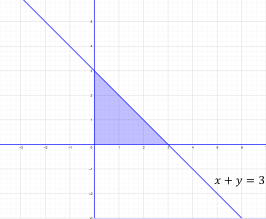
\includegraphics[scale = ]{img/tri.png}
  \end{center}
\end{esempio}
Si possono avere problemi con regione non ammissibile, ovvero con
$X=\emptyset$, che implica che il problema è mal posto oppure bisogna
abbassare qualche vincolo. Si può avere un problema illimitato con:
\[\forall c \in \mathbb{R}\exists x_c\in X:f(x_c)\leq c\,\, se\,\,
  opt = min\]
\[\forall c \in \mathbb{R}\exists x_c\in X:f(x_c)\geq c\,\, se\,\,
  opt = max\]
Infine si può avere una sola soluzione ottima o più (anche infinite)
soluzioni ottime utte con lo stesso valore della funzione
obiettivo.
\begin{esempio}
  abbiamo la funzione obiettivo
  \[\min_{x,y}(x^2+y^2)\]
  con i 3 vincoli:
  \[x+y \leq -1\]
  \[x\geq 0\]
  \[y\geq 0\]
  Non ha soluzione (è matematicamente impossibile) e il problema
  non è ammissibile
\end{esempio}
\begin{esempio}
  abbiamo la funzione obiettivo
  \[\max_{x,y}(x^2+y^2)\]
  con i 2 vincoli:
  \[x\geq 0\]
  \[y\geq 0\]
  Ha come soluzione infinito
\end{esempio}
\begin{esempio}
  abbiamo la funzione obiettivo
  \[\max_{x,y,z}(z)\]
  con i 4 vincoli:
  \[x+y+z = 2\]
  \[0\leq x \leq 1\]
  \[0\leq y \leq 1\]
  \[0\leq z \leq 1\]
  Ha infinite soluzioni (tutte le soluzioni con $z=1$ e $x+y=1$, in quanto cerco
  il max di z e come ultio vincolo ho che al massimo è 1)
  \begin{center}
    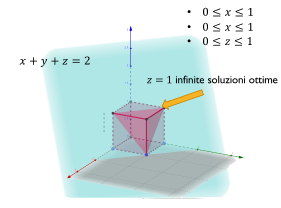
\includegraphics[scale = 1]{img/tri2.png}
  \end{center}
\end{esempio}
La risoluzione di un problema di Programmazione matematica consiste
nel trovare una soluzione ammissibile che sia un \textbf{ottimo
  globale} ovvero un vettore $^*\in X$ tale che:
\[f(x^*)\leq f(x)\,\,\forall x\in X\,\,se\,\,opt=\min\]
\[f(x^*)\geq f(x)\,\,\forall x\in X\,\,se\,\,opt=\max\]
Quando il problema è molto difficile da risolvere possiamo
accontentarci di un ottimo locale, vale a dire un $\hat{x}\in X$ tale
che, fissato un $\varepsilon > 0$ opportuno si ha che (per problemi di
minimo e massimo):
\[f(\hat{x})\leq f(x)\,\,\forall x\in X:\,\||x-\hat{x}||\leq
  \varepsilon\,\,se\,\,opt=\min\]
\[f(\hat{x})\geq f(x)\,\,\forall x\in X:\,\||x-\hat{x}||\leq \varepsilon\,\,se\,\,opt=\max\]
Un problema di ottimizzazione può avere più ottimi locali e globali e
i punti di ottimo globale sono anche di ottimo locale.
\begin{center}
  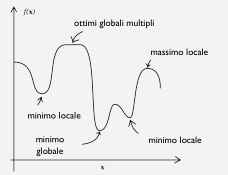
\includegraphics[scale = 1.3]{img/opt.png}
\end{center}
\newpage
\begin{esempio}
  abbiamo la funzione obiettivo:
  \[\min_{x,y}((x-0.2)^2+y^2)\]
  con i 3 vincoli:
  \[x+y \leq 1\]
  \[x\geq 0\]
  \[y\geq 0\]
  In viola si ha la funzione obiettivo tridimensionale e convessa
  e in azzurro la regione ammissibile
  \begin{center}
    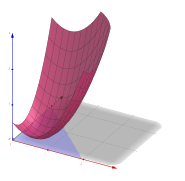
\includegraphics[scale = 1.3]{img/optes.png}
  \end{center}
  si ha solo un minimo globale.
  Si possono usare le \textbf{curve di livello} che sono le proiezioni
  ortogonali sul piano cartesiano ottenute intersecando il piano z con
  il grafico della funzione.\\
  In generale si useranno tecniche numeriche anche se si ha che
  \textbf{una funzione convessa ha un solo minimo globale}
\end{esempio}
\newpage
\begin{esempio}
  abbiamo la funzione obiettivo:
  \[\min_{x}(0.2x^2+(1-\cos(\pi x)))\]
  con i 2 vincoli:
  \[x\geq 5\]
  \[y\geq 0\]
  e si ha il seguente grafico:
  \begin{center}
    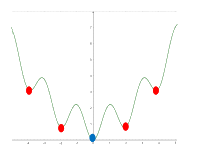
\includegraphics[scale = 1.3]{img/optes2.png}
  \end{center}
  si ha il coseno quindi si ha una funzione nè concava nè convessa
  si ha quindi un ottimo globale e 4 locali
\end{esempio}
Si ha:
\begin{itemize}
  \item \textbf{programmazione lineare (PL)}, con obiettivo e vincoli
  lineari:
  \[opt\,f(x)=c^T x\]
  \[X=\{x\in\mathbb{R}^n:\, g_i(x)\{\leq, =, \geq\}0,\,\,
    i=1,\ldots m\,\, g_i(x)=a_i^T x-b_i\}\]
  \item \textbf{programmazione lineare intera (PLI)}, con obiettivo e
  vincoli lineari interi:
  \[opt\,f(x)=c^T x\]
  \[X=\{x\in\mathbb{Z}^n:\, g_i(x)\{\leq, =, \geq\}0,\,\,
    i=1,\ldots m\,\, g_i(x)=a_i^T x-b_i\}\]
  \item \textbf{programmazione non lineare (PNL)}, con obiettivo e
  vincoli $g_i(x)$ non lineari:
  \[opt\,f(x)\]
  \[X=\{x\in\mathbb{R}^n:\, g_i(x)\{\leq, =, \geq\}0,\,\,
    i=1,\ldots m\,\, g_i(x)=a_i^T x-b_i\}\]
\end{itemize}
\begin{esempio}
  abbiamo la funzione obiettivo:
  \[\min_{x,y}(x^2+y^2)\]
  con i 3 vincoli:
  \[x+y\leq 1\]
  \[x\geq 0\]
  \[y\geq 0\]
  non è lineare in quanto x e y sono al quadrato e quindi non lineare
\end{esempio}
\begin{esempio}
  abbiamo la funzione obiettivo:
  \[\min_{x,y}(x+y)\]
  con i 2 vincoli:
  \[x^2-1\geq 0\]
  \[y\geq 0\]
  non è lineare in quanto ho un vincolo al quadrato e quindi non
  lineare 
\end{esempio}
\begin{esempio}
  abbiamo la funzione obiettivo:
  \[\min_{x,y}(x+4y)\]
  con i 4 vincoli:
  \[x+y=3\]
  \[x^2-1\geq 0\]
  \[x\geq 0\]
  \[y\geq 0\]
  non è lineare in quanto ho un vincolo al quadrato e quindi non
  lineare ma posso renderlo lineare in quanto $x^2-1=(x-1)(x+1)$ ma
  $x+1$ è sempre positivo quindi posso ammorbidire il vincolo
  rendendo il problema lineare
\end{esempio}
\begin{esempio}
  \begin{center}
    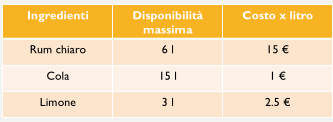
\includegraphics[scale = 0.7]{img/cub.png}
  \end{center}
  Le dosi ideali sono: almeno il 25\% di rum (R) chiaro e il 50\% di
  Cola (C) e non più del 10\% di limone (L) e voglio 10L di cubalibre. Abbiamo quindi, per logica:
  \[R\geq 0\]
  \[C\geq 0\]
  \[L\geq 0\]
  \[R\leq 6\]
  \[C\leq 15\]
  \[L\leq 3\]
  quindi:
  \[0\leq R\leq 6\]
  \[0\leq C\leq 15\]
  \[0\leq L\leq 3\]
  inoltre:
  \[R+C+L\geq 10\]
  che è:
  \[R+C+L -10\geq 0 = \left[
      \begin{matrix}
        1 & 1 & 1
      \end{matrix}
    \right]\left[
      \begin{matrix}
        R \\
        C \\
        L
      \end{matrix}
    \right] -10 \geq 0\]
  quindi:
  \[a_1^T= \left[
      \begin{matrix}
        1 & 1 & 1
      \end{matrix}
    \right], \,x =\left[
      \begin{matrix}
        R \\
        C \\
        L
      \end{matrix}
    \right],\, b_1=10 \]
  Cosa vuol dire almeno il 25\% di rum chiaro?
  \[R \geq 0.25 \cdot (R + C + L)\]
  Cosa vuol dire almeno il 5o\% di cola?
  \[R \geq 0.5 \cdot (R + C + L)\]
  Cosa vuol dire almeno il 25\% di limone?
  \[R \geq 0.1\cdot (R + C + L)\]
  che sono vincoli lineari.\\
  quindi il costo è:
  \[\min_{R,C,L}(15R+C+2.5L)\]
  che è una funzione obiettivo lineare.\
  Osserviamo che la funzione obiettivo può essere scritta anche nella
  seguente forma compatta:
  \[\min c^tx,\,\,con\,\,c^t=\left[
      \begin{matrix}
        15 & 1 & 2.5
      \end{matrix}
    \right]\,\,e\,\, x =\left[
      \begin{matrix}
        R \\
        C \\
        L
      \end{matrix}
    \right] \]
  Ora riscriviamo in forma matriciale:
  \[\min cx\]
  \[Ax\geq b\]
  \[x\geq 0\]
  con:
  \[c=\left[
      \begin{matrix}
        15 & 1 & 2.5
      \end{matrix}
    \right]\]
  \[x =\left[
      \begin{matrix}
        R \\
        C \\
        L
      \end{matrix}
    \right]\]
  la prima riga sarà $R+C+L\geq 10$\\
  la seconda sarà $R\geq 0.25\cdot (R+C+L) \geq 0 \to
  (1-0.25)R-0.25R-0.25L$\\
  la terza sarà $C\geq 0.5\cdot (R+C+L) \geq 0 \to
  -0.5R + (1-0.5)C-0.5L$\\
  la quarta sarà $L\geq 0.1\cdot (R+C+L) \geq 0 \to
  -0.1R -0.25C +0.9(1-0.1)L$\\
  la quinta sarà $0 \leq R \leq 6 \to -R \geq -6$\\
  la sesta sarà $0 \leq C \leq 15 \to -C \geq -6$\\
  la settima sarà $0 \leq L \leq 3 \to -L \geq -6$\\
  e quindi:
  \[Ax=\left[
      \begin{matrix}
        1 & 1 & 1 \\
        0.75 & -0.25 & -0.25 \\
        -0.5 & 0.5 & -.5 \\
        0.1 & 0.1 & -0.9 \\
        -1 & 0 & 0 \\
        0 & -1 & 0 \\
        0 & 0 & -1
      \end{matrix}
    \right]
    \left[
      \begin{matrix}
        R \\
        C \\
        L
      \end{matrix}
    \right] \geq
    \left[
      \begin{matrix}
        10 \\
        0 \\
        0 \\
        0 \\
        -6 \\
        -15 \\
        -3 
      \end{matrix}
    \right]\]
\end{esempio}

\begin{esempio}
  Si ha che:
  \begin{center}
    
\includegraphics[scale = 0.7]{img/steam.png}
  \end{center}
  Il comprare o no un videogioco può essere modellizzato per mezzo
  di variabili decisionali binarie associate ad ogni gioco usando
  variabili binarie:
  \[x_i\in\{0,1\}\,i=1,\ldots n\]
  con $x_i=1$ si compra con $x_i=0$ no.\\
  Non superare il budget massimo di 100 euro può essere espresso
  dalla seguente relazione:
  \[39,99 \cdot x_1 + 39,99 \cdot x_2 + 59,99 \cdot x_3 + 59,99 \cdot
    x_5 + 19,99 \cdot x_5+ 29,99 \cdot x_6 ≤ 150\]
  Non superare la memoria massima può essere espresso dalla seguente
  relazione:
  \[30 \cdot x_1 + 40 \cdot x_2 + 12 \cdot x_3 + 46 \cdot
    x_5 + 12 \cdot x_5+ 70 \cdot x_6 ≤ 150\]
  e sono vincoli lineari.\\
  Volere i giochi che più ci piacciono si esprime nel seguente modo:
  \[\max(2\cdot x_1+5\cdot x_2+2\cdot x_3+5\cdot x_4+3\cdot x_5+5\cdot x_6)\]
  che è una funzione obiettivo lineare.\\
  Volere i giochi che più ci piacciono, avendo 200 euro di budget e
  100GB si spazio corrisponde a:
  \[\max(2\cdot x_1+5\cdot x_2+2\cdot x_3+5\cdot x_4+3\cdot x_5+5\cdot x_6)\]
  \textbf{Si tratta, quindi, di un problema di programmazione lineare a
    variabili binarie, che sono un caso particolare di variabili
    intere}.\\
  \textbf{\textit{Un modello di ottimizzazione di questo tipo prende
      il nome di Problema dello zaino (Knapsack)}}
\end{esempio}
\textbf{altri esempi sulle slide}
\begin{esempio}
  Partendo dai dati di vendita di avatar capire se Endgame supererà gli
  incassi di avaatar, sapendo gli incassi dei primi giorni.\\
  Vogliamo costruire una retta di regressione lineare che interpoli i
  dati:
  \[y=ax+b,\,\,a,b\in\mathbb{R}\]
  Bisogna calcolare la retta di regressione corrisponde al seguente problema di
  ottimizzazione non vincolata:
  \[\min_{a,b}\left[\frac{1}{2}\sum_{i=1}^n (y_i-ax_i-b)^2\right]\]
  e quindi si ha funzione obiettivo non-lineare con $a,b$ variabili
  continue. Cerco quindi la retta di regressione partendo dai primi dati
  e ipotizzo una previsione e cerco $a$ e $b$
  :
  \begin{center}
    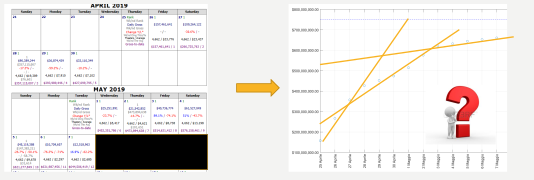
\includegraphics[scale = 0.9]{img/prev.png}
  \end{center}

  \begin{center}
    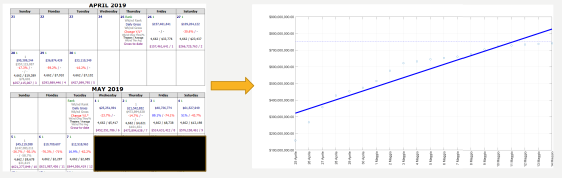
\includegraphics[scale = 0.9]{img/prev2.png}
  \end{center}
  \textbf{Questo è un problema di ottimizzazione non vincolata e non lineare}
\end{esempio}
\textbf{altri esempi sulle slide}
\begin{comment}
  \subsection{Esercizio}
  \begin{esercizio}
    \textbf{testo:}\\
    \textit{La Svivon produce  batterie  elettriche  di  tre  tipi
      (Alfa,  Beta  e  Gamma).  Per  due  di  esse  (Beta  e  Gamma)
      utilizza del rame. Per coprire la produzione del prossimo mese, può
      acquistare il rame al prezzo di 5 euro/kg. Il fornitore però non
      può fornire più di 4000  kg  di rame.  Nella  seguente  tabella
      sono  indicate: la  quantità di  rame  richiesta  per  ciascuna
      batteria, i costi di manodopera (per batteria prodotta) e prezzi
      di vendita al pubblico (per batteria):}
    \begin{center}
      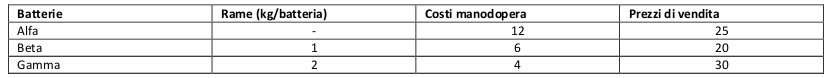
\includegraphics[scale = 0.7]{img/es1.png}
    \end{center}
    \textbf{(costi e manodopera sono entrambi in euro/batteria)}\\
    \textbf{Si suppinga che ogni batteria prodotta sia anche venduta.}\\
    \textit{I tre tipi di batteria vogliono essere prodotti in quantità
      tali che il numero di batterie di tipo Alfa sia almeno doppio del
      numero  di  batterie  di  tipo  Beta  e  non  superiore  al
      numero di  batterie  Gamma.  Formulare un  opportuno  modello
      di programmazione lineare per la pianificazione ottimale
      dell’attività diproduzione della Svivon.}\\
    \textbf{Soluzione:}\\
    Innazitutto partiamo dal'ultima frase e definiamo le relazioni tra i
    tipi di batteria. Definiamo $x_i$ il numero di batterie di tipo
    $i\in I$, con   $I=\{\alpha, \beta, \gamma\}$ \textbf{insieme degli
      indici}. Cerchiamo ora funzione \textbf{obiettivo} e
    \textbf{vincoli}.\\
    Suppongo di produrre una batteria di tipo $\alpha$, avrò un guadagno
    effettivo pari a guadagno meno costi: $25-12=13$. Per le $\beta$ si
    avrà, avendo anche il costo del rame di 5 euro al kilo, $20-6-5\cdot
    1= 9$. Per le $\gamma$ sarà $30-4-5\cdot 2 = 16$. L'azienda
    ovviamente vuole guadagnare di più, dobbiamo massimizzare il
    profitto. Il profitto delle $\alpha$ sarà $13x_\alpha$, per le
    $\beta$ sarà $9x_\beta$ e per le $\gamma$ sarà $16x_\gamma$.
    Quindi si avrà la seguente funzione obiettivo:
    \[\max(z) = 13x_\alpha+ 9x_\beta +16x_\gamma\]
    con i seguenti vincoli (ricordando che solo le $\beta$ e le $\gamma$
    usano il rame):
    \[
      \begin{cases}
        x_\alpha \geq 2x_\beta \\
        x_\alpha \leq x_\gamma \\
        x_\beta +2x_\gamma < 4000
      \end{cases}
    \]
    Bisogna specificare che le variabili non sono continue, quindi
    aggiungiamo un vincolo di interezza:
    \[x_i\in\mathbb{N},\, \forall i\in I\]
    E abbiamo risolto le richieste dell'esercizio
  \end{esercizio}
  \begin{esercizio}
    \textbf{Testo:}\\
    \textit{Un’industria con dueimpianti  produttivi  localizzati  a
      Rimini e Firenze è interessata a sapere qual è l’organizzazione
      ottimale della propria rete distributiva, in modo da ottimizzare
      la consegna dei prodotti presso letreprincipali città di
      distribuzione:Palermo, Milano  e Roma.  La  capacità  produttiva
      dei  due  impianti  di  produzione  è  la  seguente: Rimini 300,
      Firenze 600. La domanda presso le tre città di distribuzione è
      la seguente: Palermo 325, Milano 300, Roma 275. I costi associati
      al viaggio tra gli impianti di produzione e le città di
      distribuzione sono dati dalla seguente tabella:}
    \begin{center}
      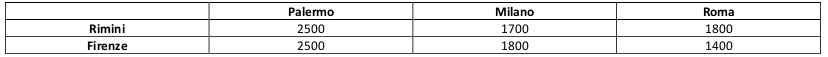
\includegraphics[scale = 0.7]{img/es3.png}
    \end{center}
    \textit{Formulare un modello di Programmazione lineare che
      permetta di pianificare lo spostamento ottimale dei prodotti
      dagli impiantialle cittàdi distribuzione in modo tale da
      minimizzare i costi di viaggio}\newpage
    \textbf{Soluzione:}\\
    \begin{center}
      \begin{tikzpicture}[shorten >=1pt,node distance=7cm,on grid,auto]
        \node[state] (q_0)   {$RN (300)$};
        \node[state] (q_1) [above right =of q_0] {$PA(-325)$};
        \node[state] (q_2) [below=of q_0] {$FI(600)$};
        \node[state] (q_3) [ right =of q_2] {$MI(-300)$};
        \node[state] (q_4) [right =of q_0] {$RM(-275)$};
        \path[->]
        (q_0) edge  node  {$2500$} (q_1)
        (q_0) edge  node  [right = 2pt]{$1700$} (q_3)
        (q_0) edge  node  {$1800$} (q_4)
        (q_2) edge  node  {$2500$} (q_1)
        (q_2) edge  node  {$1800$} (q_3)
        (q_2) edge  node  {$1400$} (q_4);
      \end{tikzpicture}
    \end{center}
    Sugli archi ho i costi di trasporto.\\
    Definisco due insiemi indici, uno $I=\{RN,FI\}$ con le città di
    partenza, e uno $J=\{PA, MI, RM\}$ con le città d'arrivo. \\
    Quindi le varfiabili $x_{i,j}$ indicano il numero di prodotti
    trasportati da dalla città $i\in I$ a quella $j\in J$.\\
    Avrò la seguente funzione obiettivo:
    \[\min(z)= 2500x_{RN, PA} + 1700x_{RN, MI}+\cdots + 1400x_{FI,RM}\]
    che può essere scritta in maniera compatta definendo il dato $c_{i,j}$ come il
    costo di trasporto tra le due città $i$ e $j$, ottenendo:
    \[\min(z)=\sum_i\sum_jc_{i,j}x_{i,j}\]
    Cerchiamo ora i vincoli. A Rimini possono uscire 300 prodotti:
    \[x_{RN,PA}+x_{RN,MI}+x_{RN,RM}=300\]
    una cosa simile va fatta per Firenze.\\
    Per le città di arrivo vediamo l'esempio di Palermo:
    \[x_{RN,PA}+x_{FI_PA}=+325\]
    similmente per Milano e Roma.\\
    Questi vincoli possono essere compattati a livello di sintassi,
    indicando con $b_i$ il numero di prodotti spedibili da una città $i\in
    I$:
    \[\sum_{j\in J}x_{i,j}=b_i,\,\, \forall i \in I\]
    e indicando con $b_j$ il numero di prodotti ricevibili da una città
    $j\in J$:
    \[\sum_{i\in I}x_{i,j}=b_j,\,\,\forall j \in J\]
    e aggiungiamo il vincolo per l'interezza:
    \[x_{i,j}\in\mathbb{N},\,\,\forall (i,j)\in I\times J\]
  \end{esercizio}
\end{comment}
\section{Soluzione Grafica}
Consideriamo un problema di programmazione lineare. Abbiamo la
seguente funzione obiettivo:
\[opt\,f(x)=c^Tx\]
con i seguenti vincoli lineari:
\[X=\left{x\in\mathbb{R}^n:\, g_i(x)\{\leq, =, \geq\}0,\, i=1\ldots
      m\right}\]
con:
\[g_i(x)=a_i^Tx-b_i,\,\, a\in \mathbb{R}, b\in \mathbb{R}^m,\,\, c\in
  \mathbb{R}^n,\,\,opt=\{min, max\}\]
I problemi di ottimizzazione reali si presentano in forma PL se sono
verificate le seguenti ipotesi:
\begin{itemize}
  \item \textbf{proporzionalità:} il contributo di ogni variabile
  decisionale al valore della funzione obiettivo è proporzionale
  rispetto al valore assunto dalla variabile stessa
  \item \textbf{additività:} ogni funzione è la somma dei contributi
  delle variabili
  \item \textbf{continuità:} qualunque valore delle variabili in
  $\mathbb{R}^n$  è accettabile
\end{itemize}
\begin{shaded}
  Diamo due definizioni:
  \begin{itemize}
    \item in uno spazio euclideo un \textbf{insieme convesso} è un insieme
    nel quale, per ogni coppia di punti, il segmento che li congiunge
    è interamente contenuto nell'insieme
    \begin{center}
      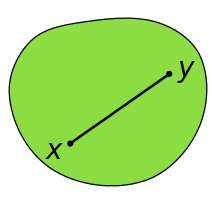
\includegraphics[scale = 0.7]{img/conv.png}
    \end{center}
    \item in uno spazio euclideo un \textbf{insieme non convesso} è un insieme
    nel quale, per ogni coppia di punti, il segmento che li congiunge non
    è interamente contenuto nell'insieme
    \begin{center}
      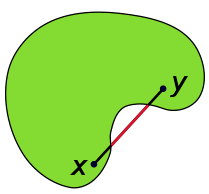
\includegraphics[scale = 0.7]{img/conc.png}
    \end{center}
  \end{itemize}
\end{shaded}
Tornando al problema iniziale iniziamo a studiare il caso
\textbf{2D}. In questo caso si ha che:
\begin{itemize}
  \item i vinvoli $g_i(x)$ possono essere rette (se $g_i(x)=0$) o
  semipiani (se $g_i(x)\neq 0$)
  \item la regione ammissibile $X$ risulta essere un sottoinsieme
  convesso del piano cartesiano
  \item la funzione obiettivo $z=c_1x_1+c_2x_2$ è un piano nello
  spazio $\mathbb{R}^3$
\end{itemize}
\textit{assumiamo inoltre, senza perdere generalità, un vincolo di
  non negatività delle variabili, ovvero $x_1,x_2\geq 0$}.\\
Un vincolo del tipo $a_1x_1+a_2x_2=b_1$ è una retta nel piano, con
l'inclinazione che è perpendicolare al vettore $v=(a_1,a_2)$:
\begin{center}
  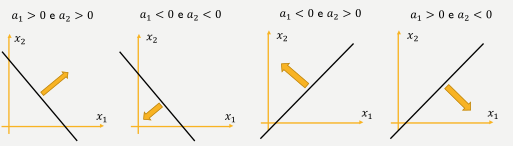
\includegraphics[scale = 0.7]{img/2d.png}
\end{center}
Questo viene detto \textbf{vincolo retta}.\\
Studiamo ora il \textbf{vincolo semipiano}, che è un vincolo del tipo
$a_1x_1+a_2x_2\leq b_1$ (che è appunto un semipiano).
\begin{shaded}
  Per disegnare il semipiano disegnamo prima la retta associata
  $a_1x_1+a_2x_2=b_1$. Scegliamo poi un punto non appartenente a tale
  retta e:
  \begin{itemize}
    \item se il punto verifica la disuguaglianza allora scegliamo il
    semipiano che lo contiene
    \item altrimenti scegliamo un altro semipiano
  \end{itemize}
  \begin{esempio}
    Si ha $x_1+x_2\leq 2$. Disegnamo quindi $x_1+x_2=2$, scegliamo il
    punto $(0,0)$ e, essendo $0+0\leq 2$ abbiamo che il punto soddisfa
    la disequazione e quindi il semipiano contiene $(0,0)$
  \end{esempio}
  \textbf{Un vincolo del tipo $a_1x_1+a_2x_2\geq b_1$ è uguale a
    $-a_1x_1-a_2x_2\leq -b_1$}
\end{shaded}
\textit{La regione ammissibile X è data dall’intersezione dei vari
  vincoli (rette e semipiani)} e quindi, dal punto di vista geometrico
corrisponde ad un \textbf{poliedro convesso} in $\mathbb{R}^2$, e può
essere limitata (\textbf{politopo}) o illimitata
\begin{center}
  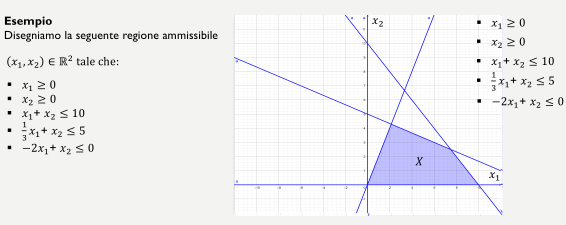
\includegraphics[scale = 0.7]{img/2d1.png}
\end{center}
\begin{center}
  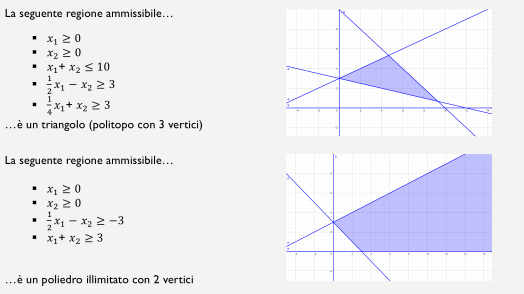
\includegraphics[scale = 0.7]{img/2d2.png}
\end{center}
\begin{esempio}
  Consideriamo il seguente problema di ottimizzazione:
  \[\maz z = -x_1+x_2\]
  con i vincoli:
  \[x_1+x_2\leq 4,\, x_1\geq 0,\, x_2\geq 0\]
  Riscriviamo la funzione obiettivo come $x_2=x_1+z$, che
  rappresenta un fascio di rette parallele al variare di $z$, che
  all'aumentare si spostano verso il punto $(0,4)$, oltre il quale si
  esce dalla regione ammissibile. Quindi la soluzione ottima è il punto
  $(0,4)$ che rappresenta un vertice della regione ammissibile (poligono
  convesso):
  \begin{center}
    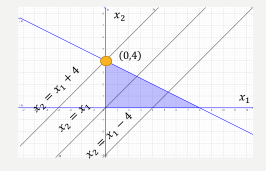
\includegraphics[scale = 0.7]{img/2d3.png}
  \end{center}
\end{esempio}
Vediamo il caso 3D.\\
la funzione obiettivo $z=c_1z_1+c_2x_2$ rappresenta un piano nello
\textbf{spazio 3D} passante per l’origine e, in particolare, se
$c_1,c_2>0$ allora il piano cresce da sinistra verso destra dal basso
verso l’alto:
\begin{center}
  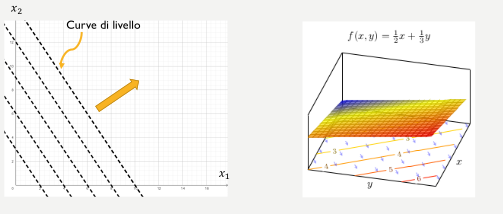
\includegraphics[scale = 0.7]{img/3d.png}
\end{center}
La funzione obiettivo $z=c_1x_1+c_2x_2$ rappresenta un piano nello
spazio 3D passante per l’origine, in particolare, se $c_1,c_2<0$,
allora il piano cresce da destra verso sinistra dall’alto verso il
basso:
\begin{center}
  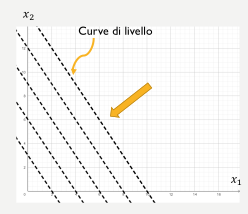
\includegraphics[scale = 0.7]{img/3d2.png}
\end{center}
Invece se $c_1>0$ e $c_2<0$ allora il piano cresce da sinistra verso
destra, dall’alto verso il basso:
\begin{center}
  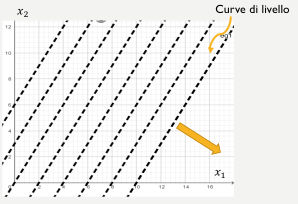
\includegraphics[scale = 0.7]{img/3d3.png}
\end{center}
Invece se $c_1<0$ e $c_2>0$ allora il piano cresce da destra verso
sinistra, dal basso verso l’alto:
\begin{center}
  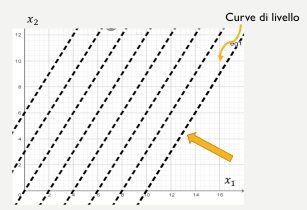
\includegraphics[scale = 0.7]{img/3d4.png}
\end{center}
\textbf{È possibile individuare il punto di massimo (minimo) del
  problema di programmazione lineare (PL) seguendo la direzione di crescita
  (decrescita) della funzione obiettivo all’interno della regione
  ammissibile}.\\
Si possono avere 3 situazioni:
\begin{enumerate}
  \item il problema PL ammette \textbf{un’unica soluzione ottima} in un
  vertice del poligono convesso che delimita la regione ammissibile
  \item il problema PL ammette \textbf{ infinite soluzioni ottime} in
  un lato del poligono convesso che delimita la regione ammissibile
  se la direzione di descrescita è perpendicolare ad un lato del
  poligono
  \item il problema PL \textbf{non ammette soluzione} perché la
  regione   ammissibile è illimitata e la funzione obiettivo
  è illimitata superiormente (se è di massimizzazione) o
  illimitata inferiormente (se è di minimizzazione)
\end{enumerate}
\begin{center}
  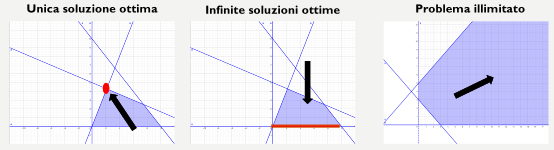
\includegraphics[scale = 0.7]{img/3d5.png}
\end{center}
\begin{esempio}
  \textbf{La società WYNDOR GLASS & Co. realizza prodotti in vetro di
    alta qualità tra cui finestre e porte in vetro. Essa possiede tre
    stabilimenti. Lo Stabilimento 1 produce telai in alluminio, lo
    Stabilimento 2 produce telai in legno, mentre lo Stabilimento 3
    produce il vetro e assembla i prodotti. I dirigenti della società
    hanno deciso di rinnovare la linea di produzione con il lancio di
    due nuovi prodotti:}
  \begin{itemize}
    \item \textbf{Prodotto 1: una porta in vetro con intelaiatura in
      alluminio}
    \item \textbf{Prodotto 2: una finestra con intelaiatura in legno}
  \end{itemize}
  \textbf{Il guadagno stimato per i due nuovi prodotti è di 3000\$ e
    5000\$ rispettivamente per lotto. Nella seguente tabella è
    rappresentato il tempo di produzione richiesto ed il tempo massimo
    disponibile per lotto nei 3 stabilimenti per i due nuovi
    prodotti:}
  \begin{center}
    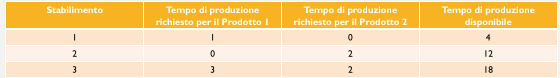
\includegraphics[scale = 0.7]{img/3d6.png}
  \end{center}
  Risolviamo usando il metodo matematico.\\
  Indichiamo con $x_1$ e $x_2$ il numero di lotti per il primo ed il
  secondo prodotto rispettivamente (\textbf{variabili
    decisionali}). Queste due variabili chiaramente non negative e
  quindi $x_1,x_2\in \mathbb{R}^+$ \textit{(anche se i lotti sono
    quantità intere in questo caso si può pensare le due quantità
    come tassi di produzione nel tempo e quindi come delle quantità
    continue)}
  Quindi si ha:
  \begin{itemize}
    \item il tempo richiesto dallo Stabilimento 1 per produrre il
    prodotto 1 è dato da $1\cdot x_1$
    \item il tempo richiesto dallo Stabilimento 2 per produrre il
    prodotto 1 è dato da $1\cdot x_2$
    \item il tempo richiesto dallo Stabilimento 3 per produrre il
    prodotto 1 e 2 è dato da $3\cdot x_1+2\cdotx_2$
  \end{itemize}
  aggiungiamo i vincoli sulle disponibilità massime di produzione:
  \[1\cdot x_1\leq 4\]
  \[2\cdot x_2\leq 12\]
  \[3\cdotx_1+2\cdot x_2\leq 18\]
  che si aggiungono a:
  \[x_1,x_2\geq 0\]
  con la funzione obiettivo, per massimizzare i profitti, che è:
  \[\max_{x_1,x_2} z = (3000\cdot x_1+5000\cdot x_2) = (3\cdot
    x_1+5\cdot x_2)\]
  ho ottenuto quindi il mio modello matematico. \textbf{Si tratta,
    quindi, di un problema di programmazione lineare a variabili
    continue con 3 vincoli (più 2 vincoli di non negatività) con la
    regione ammissibile che è un poligono convesso limitato}
  \begin{center}
    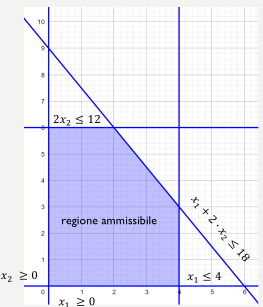
\includegraphics[scale = 0.7]{img/3d7.png}
  \end{center}
  Si ha che la funzione obiettivo crescente lungo la
  direzione positiva degli assi $x_1$ e $x_2$ e si ottiene che il valore
  che massimizza la funzione obiettivo (con $z>0$) è $(2,6)$ dove $z =
  36$.\\
  \textbf{Essendo la regione ammissibile finita e non vuota, per
    qualsiasi valore del profitto dei due prodotti si ottiene sempre
    almeno una soluzione ottima del problema (potrebbero essere
    infinite)}:
  \begin{center}
    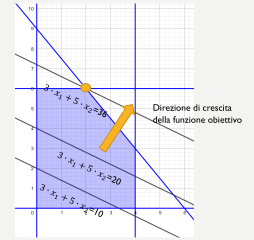
\includegraphics[scale = 0.8]{img/3d8.png}
  \end{center}
\end{esempio}

\subsection{esercizi}
\begin{esempio}
  \textbf{test:}\\
  \textit{Nell’intorno di un atomo l’energia di interazione tra
    l’atomo stesso e un altro atomo sonda che gli viene avvicinato, è
    data dalla formula}
  \[E=\frac{A}{r^{12}}-\frac{B}{r^{6^{'}}}\]
  \textit{dove A e B sono parametri caratteristici dell’atomo mentre
    rappresenta la distanza Euclidea tra l’atomo e la sonda. È data
    una  configurazione  tridimensionale  di  alcuni  atomi,  supposti
    puntiformi  e  si  vuole  trovare  il  punto  di  minima energia
    a  cui  la  sonda(anch’essa considerata puntiforme) tende a
    stabilizzarsi per  effetto  delle  interazioni  con  gli atomi
    stessi. Sono  dati  5  atomi,  posizionati  come  in  Tabella
    e  con  i  relativi  valori  di  A  e  B.  Si  vuole  determinare
    la posizione ottimale dell’atomo sonda al fine di minimizzare
    l’energia complessiva}
  \begin{center}
    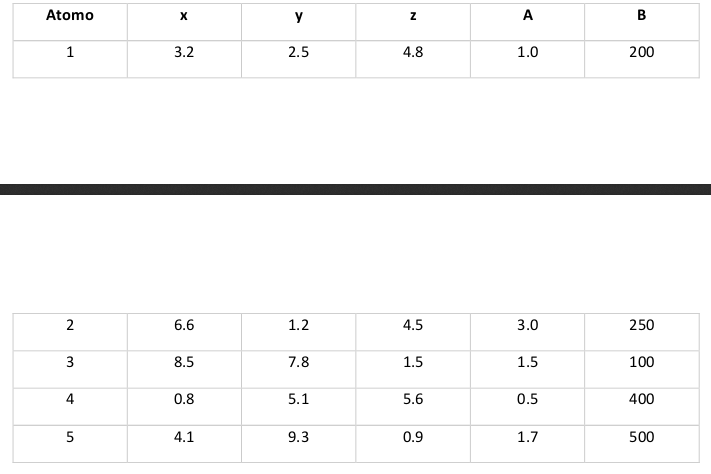
\includegraphics[scale = 0.7]{img/es.png}
  \end{center}
  \textit{Si descriva il modello matematico per esprimerela ricerca
    della soluzione di tale problema}
  \textbf{soluzione:}\\
  
\end{esempio}










\section{Simplesso}
Consideriamo nuovamente un generico problema di programmazione lineare
(PL) con la seguente funzione obiettivo lineare:
\[opt\,f(x)=C^Tx\]
con i seguenti vincoli lineari:
\[X=\left{x\in\mathbb{R}^n:\, g_i(x)\{\leq, =, \geq\}0,\, i=1\ldots
      m\right}\]
che può essere riscritto nella seguente \textbf{forma standard} (che
è un problema di massimo):
\[\max c^Tx\]
tale che $Ax=b,\, x\geq 0$, con:
\[x=\left[
    \begin{matrix}
      x_1\\
      \vdots\\
      x_n
    \end{matrix}
  \right],\,\,b=\left[
    \begin{matrix}
      b_1\\
      \vdots\\
      b_n
    \end{matrix}
  \right],\,\,A=\left[
    \begin{matrix}
      a_{11} & \cdots & a_{1n}\\
      \vdots & \ddots & \vdots\\
      a_{m1} & \cdots & a_{mn}
    \end{matrix}
  \right],\,\,c=\left[
    \begin{matrix}
      c_1 & \cdots & c_n
    \end{matrix}
  \right]\]
rispettivamente \textit{vettore colonna n × 1}, \textit{vettore colonna
  m x 1}, \textit{matrice m x n} e \textit{vettore riga m x 1}.\\
Per convenzione $b\geq 0$ quindi le $b_i$ sono positive.\\
\textbf{Ogni problema PL può essere riscritto in forma standard},
infatti:
\begin{itemize}
  \item $\min c^Tx \to -\max (-c^Tx)$ quindi esprimo un problema di
  minimo come un problema di massimo
  \item $a_i^T\leq b_i \to a_i^T+s_i=b_i$, con $s_i\geq 0$ che è è una
  nuova variabile che prende il nome di \textbf{variabile di
    slack}. Quindi esprimo un vincolo di disuguaglianza come uno di
  uguaglianza, introducendo una nuova variabile
  \item $a_i^T\geq b_i \to a_i^T-s_i=b_i$, con $s_i\geq 0$ che è è una
  nuova variabile che prende il nome di \textbf{variabile di
    surplus}. Quindi esprimo un vincolo di disuguaglianza come uno di
  uguaglianza, introducendo una nuova variabile
  \item se $x_i\in \mathbb{R}$ (variabile intera) allora si possono
  definire due nuove variabili $u_i$ e $v_i$ tali che:
  \begin{itemize}
    \item $u_i\geq 0$
    \item $v_i\geq 0$
    \item $x_i=u_i+v_i$
  \end{itemize}
  Quindi esprimo una variabile libera attraverso una combinazione
  di variabili non negative, inoltre un'altra possibilità consiste nel
  ricavare l’espressione di tale variabile da uno dei vincoli del
  problema, eliminare tale vincolo del modello e sostituire tale
  espressione laddove compaia la variabile libera.
\end{itemize}
\begin{esempio}
  \begin{center}
    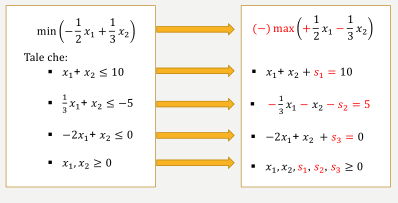
\includegraphics[scale = 0.8]{img/sim.png}
  \end{center}
  \textit{Notiamo che passiamo da un problema con 2 variabili ad
    uno con 5 variabili}
\end{esempio}
\begin{esempio}
  \begin{center}
    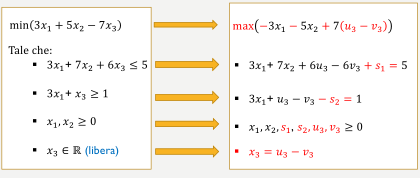
\includegraphics[scale = 0.8]{img/sim2.png}
  \end{center}
  \textit{Notiamo che passiamo da un problema con 3 variabili ad uno
    con 6 variabili. Inoltre, essendop $x_3$ libera la sostituiamo
    con $x_3 = u_3-v_3$}\\
  Possiamo anche ricavare $x_3$ dal secondo vincolo una volta
  introdotta la variabile di surplus, ottenendo $x_3=-3x_1+s_2+1$:
  \begin{center}
    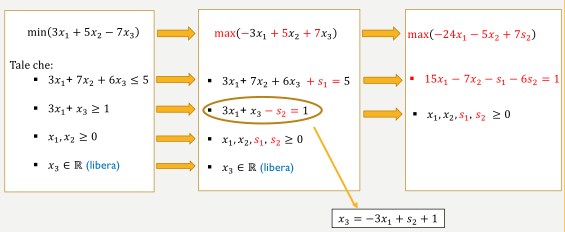
\includegraphics[scale = 0.8]{img/sim3.png}
  \end{center}
\end{esempio}
\begin{esempio}
  \textit{Riprendiamo il modello matematico relativo alla società
    Wyndor Glass Co.}:
  \begin{center}
    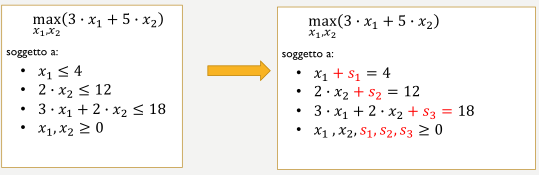
\includegraphics[scale = 0.8]{img/sim4.png}
  \end{center}
  \textit{ogni sistema di vincoli della forma $Ax \leq b$ viene
    trasformato nel sistema}:
  \[\left[
      \begin{matrix}
        A & I
      \end{matrix}
    \right]\left[
      x\\
      x_s
    \right]=b\]
\end{esempio}
con $I$ che è una matrice identità di dimensione $m\times m$ e $x_s$
sono $m$ variabili di slack.\\
Se il numero di vincoli $m$ di $A$ è strettamente maggiore del
numero di variabili $n$, allora:
\begin{itemize}
  \item se il rango di $A$ è maggiore di $n$ il sistema $Ax=b$ non
  ha soluzione, come conseguenza di Rouchè-Capelli
  \item se il rango $A$ è $n$ allora ho $m-n$ vincoli ridondanti
  \item se il numero di righe $A$ è uguale al numero di colonne
  (matrice quadrata) allora:
  \begin{itemize}
    \item se $det(A) \neq 0$ esiste un’unica soluzione del problema
    $Ax = b$. Se tale soluzione ha tutte le componenti non-negative
    allora è anche la soluzione ottimale del problema. Altrimenti
    il problema non ha soluzione
    \item se $det(A)=0$ il sistema non ammette soluzioni o uno dei
    vincoli è ridondante
  \end{itemize}
\end{itemize}
\section{Metodo del Simplesso}
Questo metodo è stato ideato da G. Dantzig nel 1947 ed è considerato
uno dei dieci migliori algoritmi del 900.\\
Questo algoritmo ha:
\begin{itemize}
  \item nel caso medio tempo computazionale lineare rispetto al numero
  delle variabili
  \item nel caso peggiore ha tempo computazionale esponenziale
\end{itemize}
È comunque uno dei più efficienti algoritmi per risolvere un problema
PL.\\
Partiamo dal solito modello matematico relativo alla società
WYNDOR GLASS \& Co:
\[\max{x_1,x_2} z= (3x_1+5x_2)\]
con:
\[x_1\leq 4,\,\,2x_2\leq 12,\,\,3x_1+2x_2\leq 18,\,\,x_1\geq 0,\,\,
  x_2\geq 0\]
\textit{che è un PL a variabili continue con 5 vincoli, 3 funzionali e
  2 di non negatività}. \textbf{Il valore che massimizza è (2,6)}
\begin{center}
  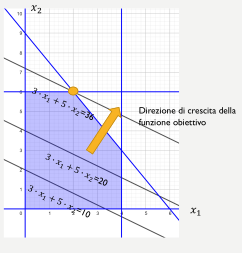
\includegraphics[scale = 0.8]{img/simp.png}
\end{center}
Partiamo ad analizzare i concetti geometrici. Per un vincolo,
l’equazione della frontiera è ottenuta sostituendo i $\geq$ e $\leq$
con $=$, otteniamo quindi:
\[x_1= 4,\,\,2x_2= 12,\,\,3x_1+2x_2= 18,\,\,x_1= 0,\,\,
  x_2= 0\]
\textbf{Ricordiamo che in due dimensioni una frontiera corrisponde ad
  una retta mentre nello spazio n-dimensionale la frontiera corrisponde ad un
  iperpiano}
\begin{center}
  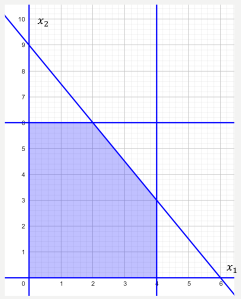
\includegraphics[scale = 0.8]{img/simp2.png}
\end{center}
Un \textbf{vertice ammissibile} è una soluzione ammissibile che non è
presente su nessun segmento che congiunge altre due soluzioni
ammissibili. \textit{i vertici di un poligono convesso non possono essere mai
  ottenuti da una combinazione convessa di altri 2 punti del
  poligono}. In 2 dimensioni ogni vertice ammissibile è
l’intersezione delle frontiere di 2 vincoli mentre in $n$ dimensioni
ogni vertice ammissibile è l’intersezione delle frontiere di n vincoli
Nell'esempio sopra si hanno 8 vertici di cui 5 ammissibili e 3 no:
\begin{center}
  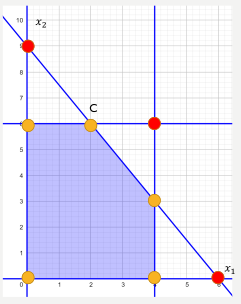
\includegraphics[scale = 0.8]{img/simp3.png}
\end{center}
e il vertice C è ammissibile ed è dato dall’intersezione
della frontiera $2x_1=12$ con $3x_1+2=18$.\\
n un problema PL 2D, due vertici si dicono \textbf{adiacenti} se
sono vertici di un medesimo segmento (la frontiera di uno dei vincoli)
della regione ammissibile.\\
\textit{Per un problema di PL con n variabili, due vertici si dicono
  adiacenti se condividono le frontiere di n − 1 vincoli. Essi sono
  collegati attraverso un segmento, chiamato \textbf{spigolo} della
  regione ammissibile}
\begin{center}
  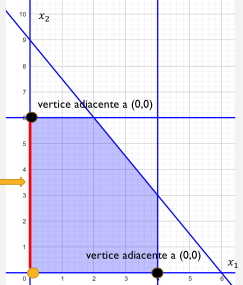
\includegraphics[scale = 0.8]{img/simp4.png}
\end{center}
Dove la linea rossa è la frontiera di $x\geq 0$.\\
Si hanno i seguenti vertici adiacenti:
\begin{center}
  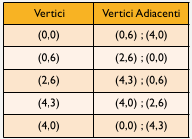
\includegraphics[scale = 0.8]{img/simp5.png}
\end{center}
Vediamo ora il \textbf{teorema fondamentale della PL}:
\begin{teorema}
  Dato un generico problema PL:
  \begin{enumerate}
    \item se esiste una sola soluzione ottima (per esempio se X è non
    vuoto e limitato), allora deve essere un vertice ammissibile
    \item se esistono soluzioni ottime multiple e la regione
    ammissibile è limitata, allora almeno due soluzioni ottime sono
    vertici adiacenti ammissibili
  \end{enumerate}
  \begin{center}
    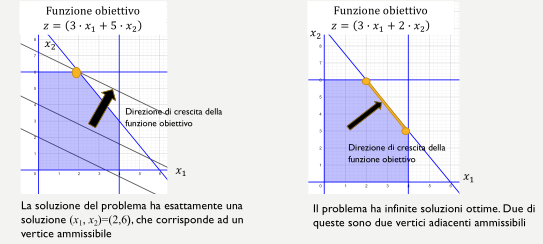
\includegraphics[scale = 0.8]{img/simp6.png}
  \end{center}
\end{teorema}
\textbf{Si ha che il numero di vertici ammissibili è finito}.\\
Nel caso in esame, questo è una conseguenza del fatto che
ogni vertice è l’intersezione di 2 delle 5 frontiere del
problema e, quindi, il numero massimo di combinazioni
differenti di 5 equazioni considerate 2 alla volta è dato da:
\[{5\choose{2}}=10\]
e nel nostro caso ne abbiamo 8 di cui 5 ammissibili.\\
\subsection{Test di Ottimalità}
i consideri un qualunque problema di PL che possieda almeno una
soluzione ottima (ad esempio se $X$ è non vuoto e limitato). Se un
vertice ammissibile non ha nessun vertice adiacente migliore
(in termini di funzione obiettivo), allora tale vertice è la soluzione
ottima.\\
Riprendendo l'esempio solito il vertice $A$ ha i due vertici adiacenti
$B$ e $E$ che sono migliori e quindi $A$ non è migliore. $C$ ha gli
adiacenti $B$ e $D$ peggiori e quindi è la souzione ottima del
problema:
\begin{center}
  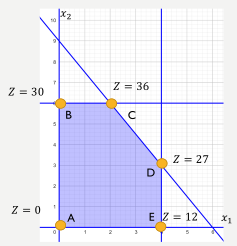
\includegraphics[scale = 0.8]{img/simp7.png}
\end{center}
Vediamo ora una simulazione del metodo del simplesso dal punto di
vista geometrico:
\begin{enumerate}
  \item \textbf{inizializzazione}, dove si sceglie (0,0) come vertice
  inziale:
  \begin{center}
    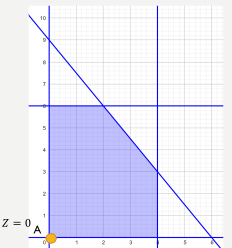
\includegraphics[scale = 0.8]{img/simp8.png}
  \end{center}
  \item \textbf{test di ottimalità:} (0,0) non è una soluzione
  ottimale ma esistono soluzioni adiacenti migliori
  \begin{center}
    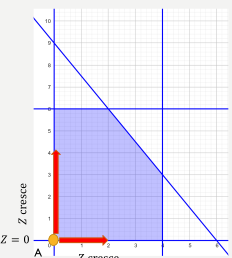
\includegraphics[scale = 0.8]{img/simp9.png}
  \end{center}
  \item \textbf{prima iterazione}, mi sposto su (0,6)
  \begin{center}
    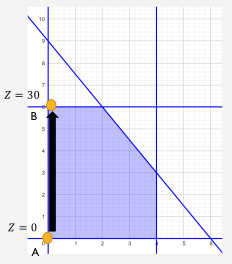
\includegraphics[scale = 0.8]{img/simp10.png}
  \end{center}
  \item \textbf{test di ottimalità:} (0,6) non è soluzione ottimale.
  Esistono soluzioni adiacenti migliori
  \begin{center}
    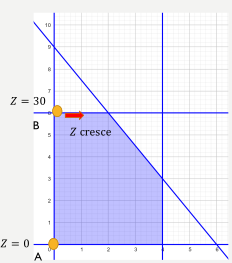
\includegraphics[scale = 0.8]{img/simp11.png}
  \end{center}
  \item \textbf{seconda iterazione}, mi sposto su (2,6)
  \begin{center}
    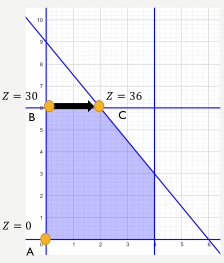
\includegraphics[scale = 0.8]{img/simp12.png}
  \end{center}
  \item \textbf{test di ottimalità}, (2,6) è la soluzione ottimale in
  quanto non esistono vertici migliori adiacenti
  \begin{center}
    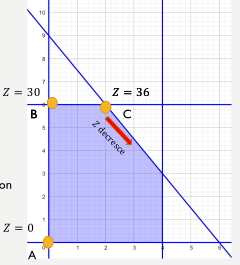
\includegraphics[scale = 0.8]{img/simp13.png}
  \end{center}
  \item \textbf{fine procedura}, termina dopo solo 2 iterazioni
  visitando 3 vertici su 5
\end{enumerate}
Questo metodo è iterativo e si concentra solo sui vertici. Se
possibile, si sceglie come vertice iniziale l’origine:
\begin{center}
  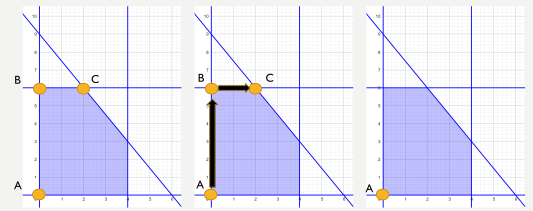
\includegraphics[scale = 0.8]{img/simp14.png}
\end{center}
Un'iterazione del metodo del simplesso corrisponde a muoversi dal
vertice corrente ad uno adiacente migliore. Il metodo del simplesso si
ferma nel momento in cui non vi sono più vertici adiacenti migliori.
\begin{center}
  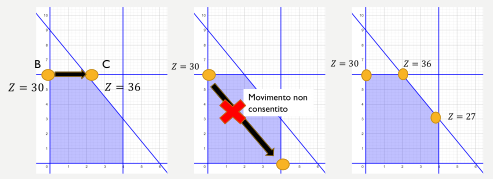
\includegraphics[scale = 0.8]{img/simp15.png}
\end{center}
Vediamo ora i \textbf{concetti algebrici del simplesso}.\\
\textit{a procedure algebrica per il metodo del simplesso, prevede di
  scrivere il problema PL in forma standard}. Considerando il solito
problema si avrebbe:
\begin{center}
  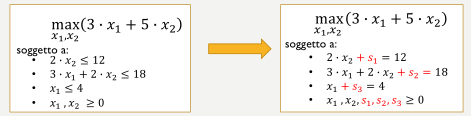
\includegraphics[scale = 1]{img/simp16.png}
\end{center}
Questa nuova forma si chiama \textbf{forma aumentata}, in quanto sin
introducono le 3 variabili $s_1, s_2, s_3$.
\newpage
Abbiamo quindi ottenuto una forma del tipo:
\[Ax=b\]
dove $A$ è una matrice $3\times 5$ e si passa da 3 a 5 variabili
(2 originali più 3 di \textit{slack}).\\
\[A=\left[
    \begin{matrix}
      0 & 2 & & 1 & 0 & 0\\
      3 & 2 & & 0 & 1 & 0\\
      1 & 0 & & 0 & 0 & 1\\
    \end{matrix}
  \right],\,\,b=\left[
    \begin{matrix}
      12\\
      18\\
      4
    \end{matrix}
  \right],\,\,x=\left[
    \begin{matrix}
      x_1\\
      x_2\\
      s_1\\
      s_2\\
      s_3
    \end{matrix}
  \right]\]
\begin{definizione}
  Una \textbf{soluzione aumentata} è una soluzione per la quale alle variabili
  originali sono aggiunte le variabili di slack e corrispodne ad una
  soluzione del sistema $Ax=b$, che è sempre risolubile fissando due
  valori di variabili.
\end{definizione}
\begin{esempio}
  Se consideriamo la soluzione 1,1 nella formulazione originale del
  problema, la soluzione aumentata è data da
  \begin{center}
    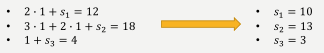
\includegraphics[scale = 1]{img/simp17.png}
  \end{center}
  Ovvero la soluzione aumentata corrisponde a $(1, 1, 10, 13, 3)$\\
  Se considero (0,8):
  \begin{center}
    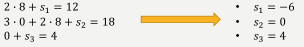
\includegraphics[scale = 1]{img/simp18.png}
  \end{center}
  Ovvero la soluzione aumentata corrisponde a $(0, 8 , −6 , 0,4)$
  (fuori da X)\\
  Se considero (4,3):
  \begin{center}
    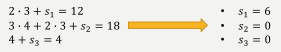
\includegraphics[scale = 1]{img/simp19.png}
  \end{center}
\end{esempio}
\begin{definizione}
  Una \textbf{soluzione di base} ammissibile è un vertice ammissibile a
  cui sono aggiunti i corrispondenti valori della variabili di slack e
  corrisponde ad una soluzione di $Ax=b$ tale che $x\geq 0$
\end{definizione}
\begin{esempio}
  consideriamo il vertice $(4,3)$ $to$ è ammissibile e la soluzione di base
  ammissibile corrispondente è $(4, 3, 6, 0, 0)$. Se considero $(4,3)$
  $to$ non è ammissibile e la soluzione di base ammissibile corrispondente
  è $(0,9,-6,0,0)$ non è ammissibile, infatti viene violato il vincolo
  di non negatività della variabile di slack $s_1$.\\
  \begin{center}
    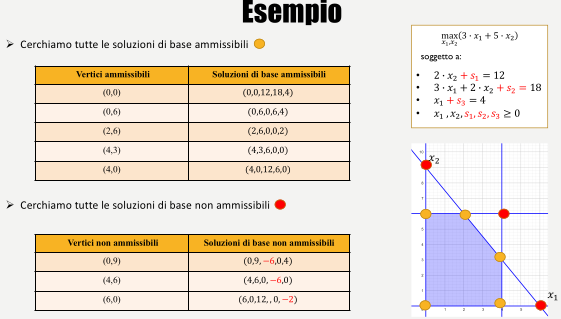
\includegraphics[scale = 1]{img/simp21.png}
  \end{center}
\end{esempio}
Una soluzione di base ha $m$ (numero dei vincoli del problema)
\textbf{variabili di base} ($\leq 0$) e le rimanenti $n − m$ ($n$ numero di
variabili della forma aumentata) sono chiamate \textbf{variabili
  non di base} ($=0$). Si ha che:
\[m\leq n\]
In una soluzione di base le variabili non di base sono nulle e i valori delle
variabili di base sono ottenuti risolvendo il sistema di $m$
equazioni.\\
\textbf{Se una delle variabili di base è nulla, si parla di 
  \textit{ soluzione di base degenere}}
\begin{definizione}
  In un problema PL due soluzioni di base si dicono adiacenti se tutte
  le variabili non di base tranne una sono uguali e questo implica che
  e variabili di base tranne una sono le stesse, anche se con 
  valori numerici differenti
\end{definizione}
\begin{center}
  \includegraphics[scale = 1]{img/simp22.png}
\end{center}
\begin{teorema}
  Dato un generico problema PL:
  \begin{enumerate}
    \item se esiste una sola soluzione ottima (per esempio se $X$ non
    è vuoto ed è illimitato) allora questa deve essere una soluzione
    di base ammissibile
    \item se esistono soluzioni ottime multiple e la regione
    ammissibile è limitata, allora almeno due soluzioni ottime sono
    soluzioni di base adiacenti ammissibili
  \end{enumerate}
  \begin{center}
    \includegraphics[scale = 1]{img/simp23.png}
  \end{center}
\end{teorema}
\textbf{Per la generazione si soluzioni di base, avendo $n$ variabili e $m$
  vincoli, si annullano $n-m$ variabili corrispondenti al numero di
  \textit{gradi di libertà}. Inoltre, in generale, il numero di
  combinazioni defferenti considerate $m$ alla volta è:}
\[{n\choose m}=\frac{n!}{m!(n-m)!}\]
Usiamo un criterio per generare le soluzioni di base, ovvero ci
spostiamo lungo i confini della regione ammissibile. I coefficienti della
variaboli non di base indicano il \textbf{tasso di miglioramento}
prodotto da un eventuale aumento del valore di
tali variabili dai valori correnti. Si hanno quindi $n-m$ tassi di
miglioramento e scelgo sempre il tasso di miglioramento maggiore (se
cerco il massimo).\\
\textbf{Se i tassi di miglioramento relativi alle variabili non in
  base sono tutti negativi allora la soluzione di base considerata
  è ottima}.\\
\textit{Sulle slide esempio completo di uso dell'algortimo.}\\
Si hanno due casi particolari:
\begin{enumerate}
  \item \textbf{regola di Bland} per evitare il cycling.
  Per determinare la variabile uscente, nel caso in cui ci siano
  più variabili candidate ad uscire, viene selezionata quella con
  l’indice più piccolo
  \item \textbf{soluzioni ottime multiple.} Ogni qual volta un
  problema ha più di una base ottima, almeno una delle variabili non
  di base ha un coefficiente nullo nella riga della funzione
  obiettivo
\end{enumerate}
La procedura del simplesso si applica a tutti i modelli di
programmazione lineare in cui la regione ammissinbile è esprimibile
come $Ax\leq b$ con $b\geq 0$ ponendo al solito:
\[\left[
    \begin{matrix}
      A & I
    \end{matrix}
  \right]\left[
    \begin{matrix}
      x\\
      x_s
    \end{matrix}
  \right]=b
\]
con $I$ matrice identità $m\times m$ e $x_s$ che sono $m$ variabili di
stack. Scegliendo come soluzione di base iniziale
\[\left[
    \begin{matrix}
      0\\
      b
    \end{matrix}
  \right]
\]
ovvero ponendo a zero le variabili del problema originale, e $x_s=b$
\subsection{Forma Tabellare}
È la forma più semplice per rappresentare il simplesso. Si hanno .
\begin{itemize}
  \item i coefficienti delle variabili nella funzione obiettivo
  (c) cambiati di segno
  \item i termini noti delle equazioni (b)
  \item i coefficeinti delle variabili nei vincoli (A)
\end{itemize}
\newpage
Per esempio:
\begin{center}
  \includegraphics[scale = 0.8]{img/tab.png}
\end{center}
Nella prima iterazione del metodo del simplesso individuo la variabile
da far entrare in base ($x_2$)
\begin{center}
  \includegraphics[scale = 0.8]{img/tab2.png}
\end{center}
\begin{center}
  \includegraphics[scale = 0.8]{img/tab3.png}
\end{center}
Dato che il coefficeinte di $x_1$ è negativo si ha che la soluzione
non è ottimale:
\begin{center}
  \includegraphics[scale = 0.8]{img/tab4.png}
\end{center}
e proseguo così fino ad avere la soluzione ottimale, arrivando ad
avere i coefficienti di $x_4$ e $x_5$ positivi:
\begin{center}
  \includegraphics[scale = 0.8]{img/tab5.png}
\end{center}
\subsection{Forma Matriciale}
Per poter utilizzare questo metodo si parte da 2 presupposti:
\begin{enumerate}
  \item il numero di righe della matrice $A$ sia strettamente
  minore del numero di colonne ($n<m$)
  \item il rango di $A$ sia $m$
\end{enumerate}
È così sempre possibile scegleire tra le $n$ colonne di $A$ un
sottoinsieme di colonne linearmente indipendenti, ovvero una
sottomatrice quadrata invertibile:
\[B\in\mathbb{R}^{m\times m}\]
mentre le restanti $m-n$ colonne formano una sottomatrice:
\[D\in\mathbb{R}^{m\times (n-m)}\]
$B$ è detta \textbf{matrice di base} mentre $D$ \textbf{matrice non di
  base}.\\
Da una matrice $A$ possiamo estrarre al massimo:
\[{n\choose m}=\frac{n!}{m!(n-m)!}\]
\textit{ma potrebbero esserci delle $B_i$ non invertibili}.\\
vediamo un esempio:
\begin{center}
  \includegraphics[scale = 1]{img/matr.png}
\end{center}
\begin{center}
  \includegraphics[scale = 1]{img/matr2.png}
\end{center}
Data una matrice di base $B$ possiamo dividere il vettore $x$ in due
sotto-vettori:
\begin{enumerate}
  \item $x_B$ di cardinalità $m$ con variabili dette \textbf{variabili
    di base}, dove l'i-esimo  elemento è associato all'i-esima colonna di $B$
  \item $X_D$ di cardinalita $n-m$ con variaboli dette
  \textbf{variabili non di base} dove l'i-esimo elemento è associato
  all'i-esima colonna $D$
\end{enumerate}
Possiamo risolvere il sistema $Ax=b$ come:
\[
  \left[
    \begin{matrix}
      B & D
    \end{matrix}
  \right]\left[
    \begin{matrix}
      x_B\\
      X_D
    \end{matrix}
  \right]=b\longrightarrow Bx_B+Dx_D=b
\]
Essendo $B$ invertibile allora possiamo moltiplicare primo e secondo
membro dell'equazione per $B^{-1}$ ottenendo:
\[x_B+B^{-1}Dx_D=B^{-1}b\]
e ponendo $x_D=0$ si ha:
\[x_b=B^{-1}b\]
\begin{definizione}
  Dato un insieme di $m$ equazioni lineari indipendenti in $n$
  incognite che formano un sistema del tipo $Ax=b$ sia $B$ una
  qualsiasi sottomatrice $n\times m$ non singolare di $A$. Ponendo
  tutte le $n-m$ componendi di $x$ non associate a $B$ uguali a 0, la
  soluzione del restante insieme di equazioni è detta
  \textbf{soluzione di base} per il sistema $Ax=b$ ripetto alla base
  $B$. Inoltre tutte le componenti di $x$ associate alle colonne di
  $B$ sono chiamate \textbf{variabili di base}. Le soluzioni di base
  corrispondono a tutti 
\end{definizione}
Consideriamo un problema PL scritto in forma standard:
\[\max c^Tx\]
con:
\[Ax=0,\,\,\,\,\,x\geq 0\]
\begin{definizione}
  Un vettore $x$ risulta essere ammissibile se soddisfa i vincoli del
  problema PL, ovvero se $Ax=b$ e $x\geq 0$.\\
  Una soluzione di base $x$ per $Ax=b$ è detta \textbf{soluzione di
    base ammissibile (SBA)} se soddisfa i vincoli di non
  negatività. In particolare $B^{-1}b\geq 0$
  \begin{center}
    \includegraphics[scale = 1]{img/matr3.png}
  \end{center}
  Una soluzione di base $x$ per $Ax=b$ è detta \textbf{soluzione di
    base degenere} se parte delle componentid ella soluzione $x_B$ è
  nulla.\\
  Sia:
  \[\left[
      \begin{matrix}
        x_B\\
        x_D
      \end{matrix}
    \right]\]
  una soluzione del problema PL in forma standard ($\min c^Tx$, $Ax=b$
  e $x\geq 0$). Allora possiamo dividere $c$ in due sottovettori:
  \begin{enumerate}
    \item $c_B$ sotto-vettore dei coefficienti di costo associati
    alle variabili di base
    \item $c_D$ sotto-vettore dei coefficienti di costo associati
    alle variabili non di base
  \end{enumerate}
  Inoltre il valore della funzione obiettivo è dato da:
  \[c_B^TB^{-1}b\]
  in quanto:
  \begin{itemize}
    \item se $x$ è soluzione di base ammissibile allora $x_D=0$ e
    $x_B=B^{-1}b$
    \item quindi:
    \[c^Tb=[c_B|c_D]^T\left[
        \begin{matrix}
          x_B\\
          x_D
        \end{matrix}
      \right]=c_D^Tx_B+c_D^Tx_D=c_D^TB^{-1}b+c_D^T\cdot 0= c_D^TB^{-1}b\]
  \end{itemize}
\end{definizione}
\begin{teorema}
  Dato un problema PL in forma standard
  ($\min c^Tx$, $Ax=b$ e $x\geq 0$) dove $A$ è $m\times n$ di rango
  $m$ allora:
  \begin{enumerate}
    \item se esiste una soluzione ammissibile allora è soluzione
    ammissibile di base
    \item se esiste una soluzione ammissibile ottima allor aesiste una
    soluzione di base ammissibile ottima
  \end{enumerate}
\end{teorema}
Questo teorema comporta che:
\begin{itemize}
  \item la risoluzione di un problema PL continuo si riduce a cercare
  le soluzioni di base ammissibili del problema
  \item il numero di soluzioni di base possibili su $n$ variabili e
  $m$ vincoli è:
  \[{n\choose m}=\frac{n!}{m!(n-m)!}\]
  \item la soluzione ottima, se esiste, corrisponderà alla soluzione
  di base ammissibile che minimzza il problema (soddisfacendo il test
  di affidabilità)
\end{itemize}
\textbf{Questo teorema è di scarsa applicabilità a causa della
  velocità di crescita del numero delle soluzioni di base al variare
  di $n$ e $m$}
\chapter{Dualità}
Con \textit{dualità} ci si riferisce ad una diversa visione dei
problemi. Questa tecnica limita il numero di vincoli permettendo una
più facile risoluzione del problema. Il pòroblema duale fornisce
\textit{bounds} (misure(?)) utili per risolvere problemi a variabili
intere. Questa tecnica viene detta \textbf{branch and bound}. Si hanno
diversi esempi di algoritmi che usano la dualità, quali il simplesso
duale.\\
Il meccanismo consiste nell'aggiungere un secondo problema di massimo
o minimo con ulteriori vincoli.\\
Vediamo le regole per costruire il problema duale. Innazitutto vediamo
questa tabella riassuntiva:
\begin{center}
  \includegraphics[scale = 0.7]{img/dua.png}
\end{center}
\textit{ricordando che si ha un problema di massumo se i vincoli sono
  espressi con un $\leq$ e le cariabili con un $geq 0$, mentre per un
  min i vincoli sono $\geq$, con le variabili $\geq 0$}.\\
\textbf{A variabili canoniche, anticanoniche o libere del problema
  primale corrispondono vincoli canonici, anticanonici o
  all'uguaglianza del duale (e viceversa invertendo tipi di vincoli e
  tipi variabili)}:
\begin{center}
  \includegraphics[scale = 0.7]{img/dua2.png}
\end{center}
\begin{center}
  \includegraphics[scale = 0.7]{img/dua3.png}
\end{center}
\textbf{Il duale di un problema duale è il problema primale di quel
  duale.}\\
\textbf{Uno dei due problemi ha soluzione ottima sse lo ha anche
  l'altro, inoltre:}
\begin{itemize}
  \item \textbf{se un problema è possibile ma illimitato, l’altro
    problema è inammissibile}
  \item \textbf{se un problema è inammissibile, l’altro è o
    inammissibile o illimitato}
\end{itemize}
\begin{teorema}
  Il valore della funzione obiettivo per una qualsiasi soluzione
  ammissibile del problema primale (cercando il max) non può eccedere
  quello del problema duale (che cerca il min).\\
  \textit{Il valore del problema duale è un \textit{lim\_sup} del
    problema primale}.\\
  Questo è il \textbf{teorema della dualità debole}
\end{teorema}
\begin{proof}
  avendo:
  % veridicare c^T
  \[\max cx|\,\,\, Ax\leq b,\,\,x\geq 0\]
  \[\min b^Tu|\,\,\,u^TA\geq c,\,\,u\geq 0\]
  si ha che:
  \[cx\leq (u^TA)x=u^T(Ax)\leq u^Tb\]
  \[\downarrow\]
  \[cx\leq by\]
\end{proof}
\begin{teorema}
  Se esiste una soluzione ottima finita il valore ottimo della
  funzione obiettivo del problema primale è uguale a quella del duale:
  \[cx=b^Tu\]
  questo è il \textbf{teorema della dualità forte}
\end{teorema}
\begin{proof}
  Vogliamo dimostrare che se $cx^*=b^Tu^*$ allora la coppia è
  ottima. Partiamo con la dimostrazione per assurdo. Suppongo che
  $(x^*,u^*)$ non sia ottima. Esiste quindi una soluzione $x^\circ$
  ottima per cui
  \[cx^\circ \leq cx^*=b^Tu^*\]
  ma questo andrebbe in contrasto alla dualità debole e quindi è un
  assurdo
\end{proof}
vediamo i corollari, indicando con $P$ il problema primale e con $D$
il duale:
\begin{itemize}
  \item se $P(D)$ è illimitato allora $D(P)$ non è ammssibile
  \item se $P$ ha soluzione ottima finita la ha anche $D$ e viceversa
  \item se $D(P)$ non è ammissibile allora $P(D)$ è illimitato o non
  ammissibile 
\end{itemize}
\subsection{conndizioni di complementarietà}
Considero il solito PL:
\[\max cx|\,\,\, Ax\leq b,\,\,x\geq 0\]
Se questo vincolo non è attivo per una soluzione ottima $x^*$ la
corrisponden te variabile duale sarà nulla in ogni soluzione ottima
del problema duale:
\[y_i^*(b_i-\sum_{j=1}^n a_{i,j}x_j^*)=0,\,\,i=1\ldots m\]
inoltre si ha che:
\begin{itemize}
  \item se $y_i^*>0$ allora $\sum_{j=1}^n a_{i,j}x_j^*=b_j$
  \item se $\sum_{j=1}^n a_{i,j}x_j^*>b_j$ allora  $y_i^*=0$
\end{itemize}
quindi per:
\[\max cx|\,\,\, Ax\leq b,\,\,x\geq 0\]
\[\min b^Tu|\,\,\,u^TA\geq c,\,\,u\geq 0\]
si ha:
\begin{itemize}
  \item $u_j^{*T}(b_J-A_jx^*)=0,\,\,\forall j$
  \item $(u^{*T}A_i-c_i)x^*=0,\,\,\forall i$
\end{itemize}
Nel complesso si ha che: \textbf{il vettore della variabili duali
  ottime per un problema di PL è $c_bb^{-1}$ ed è visualizzabile se si
  usa il tableau:}
\begin{center}
  \includegraphics[scale = 0.7]{img/dua4.png}
\end{center}
\subsection{Analisi di Sensività}
Ci si propone di studiare gli effetti sulla soluzione ottima in
seguito alle modifiche di parametri del modello (dei vettori $b$ o dei
coefficienti $c$).\\
Prendendo un qualsiasi problema di PL si arriva, ipotizziamo di
variare il coefficiente di uno dei vincoli di un certo $\Delta
c$. Arriveremo ad un tableau finale della forma:
\begin{center}
  \includegraphics[scale = 0.7]{img/add.png}
\end{center}
e il valore $c_bB^{-1}$ viene definito \textbf{prezzo ombra}, ovvero
tasso di variazione della funzione obiettivo al variare (limitato)
del termine noto e corrispondono alla soluzione ottima del problema
duale.\\
Si definisce l'\textbf{intervallo ammissibile per la base ottima}
l'intervallo di valori per cui la soluzione di base ottima corrente
rimane ammissibile. L'effetto su $z$ del cambiamento di $b_i$ dato dal
prezzo ombra continua ad essere valido a condizione che i valori di
$b_i$ rimangano all'interno di questo intervallo.\\
Il cambiamento nel vettore risorse si rappresenta con:
\[b_i\to b_i+\delta\]
e il prezzo ombra di un vincolo può essere visto come il tasso di
miglioramento della funzione obiettivo all'aumentare del termine noto
di quel vincolo. Inoltre le condizioni di ottimalità non sono affette
dalla variazione indicata ma basta verificare
l'\textbf{ammissibilità}:
\[B^{-1}(b+\delta e_i)\geq 0\Longrightarrow B^{-1}b+b^{-1}e_i\geq
  0\Longrightarrow x_b+g\geq 0\]
con $g$ è l'i-sima colonna di $B^{-1}$. Quindi per avere una soluzione
ammissibile mi serve un $\delta$ tale che:
\[\min_{g_i<0}\frac{-x_i}{g_i}\geq \delta \geq \max_{g_i<0}\frac{-x_i}{g_i}\]
E si ottiene la seguente variazione della funzione obiettivo:
\[c_BB^{-1}(b+\delta e_i)=C_BB^{-1}b+C_BB^{-1}\delta e_i\]
% non ho capito

\subsection{Regola del 100\%}
\begin{definizione}
  I prezzi ombra rimangono validi per la predizione dell'effetto di
  una modifica simulatenea di più termini noti dei vincoli se questi
  cambiamenti non sono troppo grandi. Se la somma delle percentuali
  dei cambiamenti rispetto ai propri intervalli con ottimalità supera
  il 100\% allora i prezzi ombra resteranno validi
\end{definizione}
\begin{esempio}
  Sia $\max_{x_1,x_2}z=3x_i+5x_2$ con:
  \[
    \begin{cases}
      x_1\leq 4\\
      2x_2\leq 12\\
      3x_1+2x_2\leq 18\\
      x_1,\,x_2\geq 0
    \end{cases}
  \]
  e cambiamo $b_2$ da 12 a 24. Si arriv al seguente tableau finale:
  \begin{center}
    \includegraphics[scale = 0.7]{img/add2.png}
  \end{center}
  quindi:
  \begin{center}
    \includegraphics[scale = 0.7]{img/add3.png}
  \end{center}
  e $b_3$ avrà il seguente intervallo di variazione:
  \begin{center}
    \includegraphics[scale = 0.7]{img/add4.png}
  \end{center}
  Supponiamo ora di voler aumentare $b_2$ a 15 e diminuire $b_3$ a
  15. Si ha che:
  \begin{center}
    \includegraphics[scale = 0.6]{img/add5.png}
  \end{center}
\end{esempio}
\textbf{proseguire}
\chapter{Programmazione Lineare Intera}
Sia:
\[opt\,f(x)=c^Tx\]
con i seguenti vincoli lineari:
\[X=\left{x\in\mathbb{R}^n:\, g_i(x)\{\leq, =, \geq\}0,\, i=1\ldots
      m\right}\]
con:
\[g_i(x)=a_i^Tx-b_i,\,\, a\in \mathbb{R}, b\in \mathbb{R}^m,\,\, c\in
  \mathbb{R}^n,\,\,opt=\{\min, \max\}\]
Si hanno tre divisioni:
\begin{enumerate}
  \item se $x\in \mathbb{Z}^n$ si ha un problema di
  \textbf{programmazione lineare intera, \textit{PLI}}
  \item se $x\in \{0,1\}^n$ si ha un problema di
  \textbf{programmazione lineare binaria, \textit{PB}}
  \item se $x\in \mathbb{R}^p\mathbb{Z}^q$, con
  $p+q=n,\,\,p>0,\,\,q>0$, si ha un problema di \textbf{programmazione
    lineare mista, \textit{PLM}}
\end{enumerate}
Un PLI ha un numero di soluzioni inferiori a quelle di un PL e, nel
momento in cui si ha una regione ammissibile limitata, si ha per forza
un numero di soluzioni ammissibili finito. Purtroppo questo non
implica che sia semplice trovare le soluzioni di un PLI.\\
Per esempio, avendo un PLI con $n=20$ variabili binarie ho $2^{20}$
soluzioni possibili. \\
Si cerca quindi un metodo per formulare il corrispettivo PL di un PLI,
ovvero lo stesso problema ma senza i problemi di interezza. Si ha il
cosiddetto \textbf{rilassamento lineare}. Vediamo due esempi.
\begin{esempio}
  Il PLI:
  \[\max z=2x_1+4x_2+3x_3\]
  coi vincoli
  \[
    \begin{cases}
      3x_1+4x_2+2x_3\leq 60\\
      2x_1+x_2+2x_3\leq 40\\
      x_1+3x_2+2x_3\leq 80\\
      x_1,x_2,x_3\in\mathbb{N}
    \end{cases}
  \]
  diventa il PL:
  \[\max z=2x_1+4x_2+3x_3\]
  coi vincoli
  \[
    \begin{cases}
      3x_1+4x_2+2x_3\leq 60\\
      2x_1+x_2+2x_3\leq 40\\
      x_1+3x_2+2x_3\leq 80\\
      x_1,x_2,x_3\geq 0
    \end{cases}
  \]
\end{esempio}
\begin{esempio}
  Il PLI:
  \[\max z=2x_1+4x_2+3x_3\]
  coi vincoli
  \[
    \begin{cases}
      3x_1+4x_2+2x_3\leq 60\\
      2x_1+x_2+2x_3\leq 40\\
      x_1+3x_2+2x_3\leq 80\\
      x_1,x_2,x_3\in\{0,1\}
    \end{cases}
  \]
  diventa il PL:
  \[\max z=2x_1+4x_2+3x_3\]
  coi vincoli
  \[
    \begin{cases}
      3x_1+4x_2+2x_3\leq 60\\
      2x_1+x_2+2x_3\leq 40\\
      x_1+3x_2+2x_3\leq 80\\
      x_1\leq 1, x_2\leq 1, x_3\leq 1\\
      x_1,x_2,x_3\geq 0
    \end{cases}
  \]
\end{esempio}
Formalizziamo questo metodo. In generale dato un PLI si ha che:
\begin{itemize}
  \item una variabile intera può essere ``rilassata'' sostituendo
  $x\in\mathbb{N}$ con $x$ variabile continua tale che $x\geq 0$
  \item una variabile binaria può essere ``rilassata'' sostituendo
  $x\in\{0,1\}$ con $x$ variabile continua tale che:
  \[
    \begin{cases}
      x\geq 0 & \mbox{vincolo di non negatività}\\
      x\leq 1 & \mbox{nuovo vincolo funzionale}
    \end{cases}
  \]
  \item una variabile intera non negativa con un vincolo del tipo
  $x\leq M$ può essere rilassata sostituendo $x\in\{o,M\}$ con $x$
  variabile continua tale che:
  \[
    \begin{cases}
      x\geq 0 & \mbox{vincolo di non negatività}\\
      x\leq M & \mbox{nuovo vincolo funzionale}
    \end{cases}
  \]
\end{itemize}
Si cerca quindi il PL di un PLI, lo si risolve e si verifica se la
soluzione sia intera. In caso contrario si ottiene un \textbf{upper
  bound} o un \textbf{lower bound} rispettivamente per problemi di
massimo o minimo. \\
Vediamo un esempio:
\begin{esempio}
  Si ha la seguente funzione obiettivo:
  \[\max z=x_2\]
  con i seguenti vincoli:
  \[
    \begin{cases}
      x_1+\frac{5}{2}x_2\leq 11\\
      x_1,x_2\in\mathbb{N}
    \end{cases}
  \]
  Si ha l'ottimo del PL (ovvero del rilassamento lineare) pari a:
  \[\left(0,\frac{22}{5}\right)\]
  e si ha che la soluzione approssimata del PLI è pari a:
  \[(0,4)\]
  ovvero $\frac{22}{5}=4,4$ viene approssimato all'intero più vicino, $4$
\end{esempio}
\textbf{Questo è un caso fortuito. Approssimare all'intero più vicino
  può portare ad una soluzione non ammissibile}.\\
Vediamo qui come ottenere la soluzione del PLI.
\subsection{Metodo Branch ad Bound}
Il metodo \textbf{Branch and Bound (\textit{B\&B})} è una tecnica
generale per la risoluzione di problemi di ottimizzazione
combinatoria (ovvero con spazio di soluzioni finito). Il B\&B è una
tecnica di \textbf{enumerazione implicita}, ovvero su provano tutte le
soluzioni fino a trovare l'ottima, scaratandone quindi alcune a priori
dimostrandone la non ottimimalità. Si basa sul \textbf{\textit{divide
    et impera}}.\\
Sia:
\[\max f(x)=c^Tx\]
con i seguenti vincoli lineari:
\[X=\left{x\in\mathbb{Z}^n:\, g_i(x)\{\leq, =, \geq\}0,\, i=1\ldots
      m\right}\]
con:
\[g_i(x)=a_i^Tx-b_i,\,\, a\in \mathbb{R}^n, b\in \mathbb{R}^m,\,\, c\in
  \mathbb{R}^n\]
questo viene definito come \textbf{problema completo}. Un PLI è un
\textbf{sotto-problema} del PL se \textit{presenta la medesima
  funzione obiettivo ma ha un sottoinsieme proprio di $X$ come regione
  ammissibile}.\\
Formalmente sia $z^*=f(x^*)$ la soluzione del problema completo e
$\widetilde{z}=f(\widetilde{x})$ la soluzione ottima di un
sotto-problema. Si ha che:
\[\widetilde{z}\leq z^*,\,\,e\,\,\,f(\widetilde{x})\leq f(x^*)\]
visto che $\widetilde{x}$ è una soluzione del problema completo.\\
\textit{Per un problema di minimo si ribaltano i $\leq$ in $\geq$}.\\
Il \textit{B\&B} usa tre teniche per risolvere un generico PLI:
\begin{enumerate}
  \item la partizione, ovvero il \textbf{branching}. Questa tecnica si
  usa per dividere un PLI $P_0$ in $k$ sotto-problemi $P_1,\ldots,
  p_k$ di modo che l'unione delle regioni ammissibili $X_1\ldots, X_k$
  dia la regione ammissibile del problema originario $X$, quindi:
  \[\bigcup_{i=1}^kP_k=P_0\]
  Si genera quindi un \textbf{albero delle soluzioni} che ha come
  radice $P_0$ e che può diramarsi iterativamente. Si ha che l'unione
  delle foglie è anche il problema $p_o$, in base ad un ragioanmento
  simile si possono avere altre unioni per ottenere $P_0$. Le
  diramazioni si hanno in base a dei vincoli (una variabile maggiore o
  minore di qualcosa etc $\ldots$).\\
  Nel caso di PB si ramifica in base ad ogni booleano di ogni
  variabile, ottenendo un albero binario.\\
  La variabile usata per il branching è detta \textbf{variabile di
    branching} che vengono utilizzate secondo l'ordine degli indici.\\
  Si hanno due modi per d:ividere l'insieme delle soluzioni
  ammissibili, fissando una variabile, per esempio $x_1$:
  \begin{itemize}
    \item fissare il valore di $x_1$ a tutti i suoi possibili valori
    \item specificare un insieme di valori per ogni nuovo sotto-problema
    che si vuole generare
  \end{itemize}
  Nel caso di PML si procede così:
  \begin{itemize}
    \item si calcola la soluzione ottima del rilassamento lineare di
    $P_0$
    \item si sceglie come variabile di branching una $x_j$ che non
    abbia valore intero nella soluzione ottima del rilassamento
    lineare
    \item si divide $P_0$ in $P_1$ e $P_2$ specificando due intervalli
    per $x_j$:
    \begin{itemize}
      \item $x_j\leq [x_j^*]$
      \item $x_j\geq [x_j^*]+1$
    \end{itemize}
  \end{itemize}
  \item la determinazione di un limite superiore, ovvero il
  \textbf{bounding}. Ad ognuno dei sotto-problemi definiti nel
  branching si può associare un bound, ovvero un limite,
  $z_1,\ldots,z_k$ su quanto buona possa essere la soluzione migliore
  di ogni sotto-problema. Questi bound si ottengono con il
  \textbf{rilassamento lineare associato}. Risolvo quindi i
  rilassamenti lineari dei sotto problemi e riporto nell'albero del
  branhcing sia la soluzione ottima che il bound (il valore di $z$) di
  ogni sottoproblema.\\
  Si definice \textbf{soluzione incombente} $x^*$ per $P_0$ la miglior (la
  più grande se ho max, la più piccola se ho min)   soluzione
  ammissibile (quindi intera) trovata finora, insieme al suo valore
  di funzione obiettivo. All'inizio si ha che $z^*=-\infty$
  \item l'eliminazione, ovvero il \textbf{fathoming}. Si ha che un
  sotto-problema $P_i$ può essere ``taglaito via'' (fathoming) e
  quindi escluso dal ragionamento se:
  \begin{itemize}
    \item il suo upper bound è $\leq z^*$. Infatti non è sicuramente
    la soluzione migliore e un suo branch non darà una soluzione
    migliore
    \item il suo rilassamento non da soluzioni ammissibili intere
    \item la soluzione ottima del rilassamento lineare è intera, in
    quanto se è migliore della soluzione incombente attuale essa
    diventa la nuova soluzione incombente (nel caso di PML basta che
    le componenti relative alla variabili intere della soluzione
    ottima siano intere)
  \end{itemize}
\end{enumerate}
Quindi, ricapitolando, per un PB si ha il seguente algoritmo
\textit{B\&B}:
\begin{shaded}
  \begin{enumerate}
    \item \textbf{inizializzazione:} si pone $z^*=-\infty$. Si fa poi
    il passo di bounding e quello di fathoming. Si esegue il test di
    ottimalità e si decide se tagliare via il problema. Se non accade
    si classifica il problema come sotto problema e si itera con
    \textit{B\&B}
    \item \textbf{iterazione del B\&B:}
    \begin{itemize}
      \item \textbf{branching:} tra i sottoproblemi rimanenti, quelli
      \textit{unfathomed} se ne sceglie uno (per esempio quello
      generato più di recente) e si generano due sotto-problemi a
      partire da esso fissando la successiva variabile di branching a
      0 o a 1
      \item \textbf{bounding:} per ogni sotto-problema ottendo il
      bound mediante il simplesso al suo rilassamento lineare
      \item \textbf{fathoming:} per ogni nuovo sotto-problema seguo i
      3 criteri per scartare quelli necessari
    \end{itemize}
    \textbf{test di ottimalità:} iterare fino ad esaurire i
    sotto-problemi. Quando smetto di iterare ho la soluzione
    incombente ottima altrimenti continuo ad iterare
  \end{enumerate}
\end{shaded}
Per un problema PLM:
\begin{shaded}
  \begin{enumerate}
    \item \textbf{inizializzazione:} si pone $z^*=-\infty$. Si fa poi
    il passo di bounding e quello di fathoming. Si esegue il test di
    ottimalità e si decide se tagliare via il problema. Se non accade
    si classifica il problema come sotto problema e si itera con
    \textit{B\&B}
    \item \textbf{iterazione del B\&B:}
    \begin{itemize}
      \item \textbf{branching:} tra i sottoproblemi rimanenti, quelli
      \textit{unfathomed} se ne sceglie uno (per esempio quello
      generato più di recente). Tra le variabili inetre che non hanno
      valore intero nella soluzione ottima del rilassamento lineare
      associato ne scelgo una come variabile di branching (per esempio
      la prima in ordine di indice) $x_j$. Sia inoltre $x_j^*$ il
      relativo valore nella soluzione ottima. Genero quindi due
      sotto-problemi aggiugendo rispettivamente i vincoli $x_j\leq
      |x_j^*|$ e $x_j\geq|x_j^*|+1$
      \item \textbf{bounding:} per ogni sotto-problema ottendo il
      bound mediante il simplesso al suo rilassamento lineare
      \item \textbf{fathoming:} per ogni nuovo sotto-problema seguo i
      3 criteri per scartare quelli necessari
    \end{itemize}
    \textbf{test di ottimalità:} iterare fino ad esaurire i
    sotto-problemi. Quando smetto di iterare ho la soluzione
    incombente ottima altrimenti continuo ad iterare 
  \end{enumerate}
\end{shaded}
\chapter{Programmazione Non Lineare}
Un \textbf{problema di programmazione non lineare \textit{PNL}} può
essere formulato da una funzione obiettivo:
\[opt\,\,f(x)\]
con $opt=\{\min,\max\}$ e soggetta ai seguenti vincoli:
\[g_j(x)\leq b_j,\,\,j=1,\ldots,m\]
\[x_i\geq 0\,\,\,i=1,\ldots,n\]
sapendo che $f:\mathbb{R}^n\to \mathbb{R}$ e $g_j:\mathbb{R}^n\to
\mathbb{R}$ sono funzioni note di $x\in \mathbb{R}^n$ (e non lineari
come in un problema PL).\\
\textit{È più frequente avere problemi non lineari che lineari.}\\
\textbf{Un problema non lineare presenta un'area ammissibile non
  delimitata da rette ma da curve e quindi l'ottimo non è più da
  cercare solo sulla frontiera.}
\\
Vediamo ora l'\textbf{ottimizzazione non vincolata in una
  variabile}.\\
Considero un PNL con la seguente funzione obiettivo da minimizzare
\[\min_{x\in\mathbb{R}}f(x)\]
la condizione sufficiente affinché $x^*$ sia il punto di minimo è che
la derivata in quel punto sia nulla (infatti in quel punto della
funzione si avrà sicuramente un punto di ottimo):
\[\frac{d\,f(x^*)}{d\,x}=0\]
Il problema è che potremmo avere a che fare con punti di ottimo locali
e non globali.\\
Studiamo quindi l'\textbf{ottimizzazione in una variabile}.\\
Considero un PNL con la seguente funzione obiettivo
\textbf{\textit{convessa}} da minimizzare:
\[\min_{x\in\mathbb{R}}f(x)\]
la condizione sufficiente affinché $x^*$ sia il punto di minimo è che:
\[\frac{d\,f(x^*)}{d\,x}=0\]
si ha quindi che:
\textit{se tale equazione può essere risolta analiticamente allora
  il procedimento per trovare l’ottimo termina.}\\
\textbf{Capire se inserire il ripasso di analisi}\\
Si hanno quindi diverse tipologie di PNL:
\begin{itemize}
  \item \textbf{ottimizzazione non vincolata:} ovvero quei problemi
  che non hanno vincoli sulla regione ammissibile e hanno la funzione
  obiettivo che è semplicemente:
  \[\max_{z\in\mathbb{R}^n}f(x)\,\,\,o\,\,\,\min_{z\in\mathbb{R}^n}f(x)\]
  \item \textbf{ottimizzazione con vincoli lineari:} ovvero i PNL che
  hanno le funzioni $g_j(x)$ lineari, pur avendo la funzione obiettivo
  non lineare. Un caso particolare è la \textbf{PNL quadratica}, che
  presenta una funzione obiettivo, appunto, quadratica
  \item \textbf{programmazione convessa:} ovvero quei PNL in cui
  $f(x)$ è concava o convessa mentre ogni funzione $g_j(x)$ è convessa
  \item \textbf{programmazione non convessa:} ovvero tutti i PNL che
  non soddisfano le ipotesi di convessità
\end{itemize}
Si quindi la funzione obiettivo una funzione concava da massimizzare:
\[\max_{x\in\mathbb{R}}f(x)\]
la condizione sufficiente per avere un punto di massimo è sempre:
\[\frac{d\,f(x^*)}{d\,x}=0\]
se posso risolvere analiticamente l'equazione ho trovato il massimo
(se fosse stata convessa il minimo). In mancanza mi affido ad
\textbf{algoritmi di risoluzione numerica}.
\begin{itemize}
  \item construisco una sequenza di punti $\{x_k\}$ tali che:
  \[\lim_{k\to +\infty}x_k=x^*\]
  \textit{ad ogni iterazione $k$, partendo da $k_k$ si esegue una
    ricerca sistematica per identificare un punto migliore $x_{k+1}$}
  \item devo garantire la convergenza della sequenza al mio punto di
  ottimo. Se la funzione è continua e concava in un intervallo $[a,b]$
  considero il genrico $x_k$:
  \begin{itemize}
    \item se $\frac{d\,f(x^*)}{d\,x}<0$ allora l'ottimo è a sinistra
    di $x_k$
     \item se $\frac{d\,f(x^*)}{d\,x}>0$ allora l'ottimo è a destra
     di $x_k$
     \item se $\frac{d\,f(x^*)}{d\,x}\approx 0$ allora l'ottimo $x_k$,
     $x_k\approx x^*$
  \end{itemize}
\end{itemize}
Non abbiamo però la certezza che un numero finito di iterazioni ci
possa portare ad un risultato. Abbiamo dei criteri per capire quando
fermarci:
\begin{itemize}
  \item come detto sopra quando la soluzione è abbastanza accurata,
  ovvero $\frac{d\,f(x^*)}{d\,x}\approx 0$
  \item quando si è raggiunto un numero massimo di iterazioni $N$
  stabilito a priori
  \item quando si hanno progressi lenti, ovvero
  $|x_{k+1}-x_k|<\varepsilon_k$ o\\ $|f(x_{k+1})-f(x_k)|<\varepsilon_f$
  \item quando la soluzione diverge, ovvero $|x_k|\to+\infty$
  \item quando si hanno dei cicli, ovvero da $x_k$ si arriva a
  $x_{k+1}$ e da $x_{k+1}$ si arriva a $x_k$ 
\end{itemize}
Si hanno due tipi di algoritmi possibili:
\begin{enumerate}
  \item \textbf{algoritmi dicotomici}, che risolvono l'equazione
  della derivata uguale a zero e ad ogni iterazione riducono
  l'intervallo di ricerca all'interno del quale la funzione derivata
  si annulla
  \item \textbf{algoritmi di approssimazione}, che usano
  approssimazioni locali della funzione
\end{enumerate}
\begin{shaded}
  Partendo dalla \textit{formula di Taylor}, centrata in $x_k$, si può
  ottenere un'approssimazione quadratica di tale funzione:
  \[f(x_{k+1})=f(x_k)+f^{'}(x_{k+1}-x_k)+\frac{1}{2}f^{''}(x_k)(x_{k+1}-x_k)^2
    +O((x_{k+1} -x_k)^2)\]
  \[\Downarrow\]
  \[f(x_{k+1})\approxf(x_k)+f^{'}(x_{k+1}-x_k)+\frac{1}{2}f^{''}(x_k)(x_{k+1}-x_k)^2\]
  Si ha che l'approssimazione quadratica è funzione solo di
  $x_{k+1}$. Calcolo quindi la derivata dell'approssimazione
  quadratica:
  \[f^{'}(x_k)+f^{''}(x_k)(x_{k+1}-x_k)=0\Longrightarrow
    x_{k+1}=x_k-\frac{f^{'}(x_k)}{f^{''}(x_k)}\]
\end{shaded}
Per l'ottimizzazione in una variabile si hanno 2 metodi:
\begin{enumerate}
  \item \textbf{metodo di bisezione}, che si applica quando $f(x)$ è
  concava, continua su un intervallo $[a,b]$ e derivabile su
  $(a,b)$.\\
  Si basa sul guardare la pendenza della funzione (ovvero la derivata)
  per un punto di $x$ per capire dove cercare il massimo (ribaltando
  nel caso du funzion e concava e ricerca del minimo):
  \begin{itemize}
    \item se $f^{'}(x)>0$ allora si può ottenere un nuovo punto
    spostandosi verso destra
    \item se $f^{'}(x)<0$ allora si può ottenere un nuovo punto
    spostandosi verso sinistra
  \end{itemize}
  inoltre, considerando un generico $x_k$:
   \begin{itemize}
    \item se $f^{'}(x_k)>0$ allora $x_k$ è un estremo inferiore
    $\underline{x}$ per $x_{k+1}$ 
    \item se $f^{'}(x_k)<0$ allora $x_k$ è un estremo superiore
    $\overline{x}$ per $x_{k+1}$ 
  \end{itemize}
  per ogni passo $k$ si identifica un \textbf{intervallo di ricerca}:
  \[[a_k,b_k]\subset[a_{k-1},b_{k-1}]\subset[a,b]\]
  per ridurre lo spazio di ricerca in modo da identificare
  un'iterazione $k$ che presenta:
  \[|b_k-a_k|<2\varepsilon\mbox{ con }|a_k-x^*|<\varepsilon \mbox{ e
    }|x^*-b_k|<\varepsilon\] 
  Vediamo ora l'lagoritmo nel dettaglio, nel caso di problema di max:
  \begin{itemize}
    \item \textbf{inizializzazione: }si fissano un $\varepsilon$ e
    $k=0$. Si calcolano $\overline{x}$ e $\underline{x}$ cercando
    valori di $x$ per cui la derivata sia positiva e negativa. Si
    sceglie il punto iniziale:
    \[x_0=\frac{\overline{x}+\underline{x}}{2}\]
    \item \textbf{iterazione del metodo della bisezione:}
    \begin{itemize}
      \item calcolo $f^{'}(x_k)$
      \item se $f^{'}(x_k)=0$ allora $x_k=x^*$
      \item se $f^{'}(x_k)<0$ allora $\overline{x}=x_k$
      \item se $f^{'}(x_k)>0$ allora $\underline{x}=x_k$
      \item infine pongo
      $x_{k+1}=\frac{\overline{x}+\underline{x}}{2}$ e $k=k+1$
    \end{itemize}
    \item \textbf{criterio d'arresto:} se
    $\overline{x}-\underline{x}\leq 2 \varepsilon$ allora $x^*$ avrà
    una distanza minore di $\varepsilon$ dall'estremo superiore (o
    inferiore). In caso contrario procedo con un'altra iterazione
  \end{itemize}
  \textbf{Il metodo di bisezione converge molto lentamente in quanto
    considera unicamente le informazioni della derivata prima}
  \item \textbf{metodo di Newton}, che si basa sull'usare l'ottimo
  dell'approssimazione quadratica di $f(x)$:
  \[x_{k+1}=x_k-\frac{f^{'}(x_k)}{f^{''}(x_k)}\]
  che è la formula che viene usata ad ogni generica iterazione $k$ per
  calcolare $x_{k+1}$.\\
  Si ha che se la funzione è concava allora $x_k$ converge verso un
  punto di massimo in quanto:
  \begin{itemize}
    \item se $f(x)$ è concava allora se $x_k$ è a sinistra del punto
    di massimo si ha che $f^{'}(x)>0$, quindi
    $-\frac{f^{'}(x_k)}{f^{''}(x_k)}>0$ e, di conseguenza,
    $x_{k+1}>x_k$
    \item se $f(x)$ è concava allora se $x_k$ è a destra del punto
    di massimo si ha che $f^{'}(x)<0$, quindi
    $-\frac{f^{'}(x_k)}{f^{''}(x_k)}<0$ e, di conseguenza,
    $x_{k+1}<x_k$
  \end{itemize}
  \textit{Se le funzione fosse stata convessa si avrebbe avuto la
    convergenza di $x_k$ verso il minimo}.\\
  Vediamo quindi nel dettaglio l'algortimo di Newton:
  \begin{itemize}
    \item \textbf{inizializzazione:} si fissa $\varepsilon$ e $k=0$
    \item \textbf{iterazione del metodo di Newton:}
    \begin{itemize}
      \item si calcolano $f^{'}(x)$ e $f^{''}(x)$
      \item si pone $x_{k+1}=x_k-\frac{f^{'}(x_k)}{f^{''}(x_k)}$
    \end{itemize}
    \item \textbf{criterio di arresto:} se $x_{k+1}-x_k|\leq
    \varepsilon$ si ha che $x_{k+1}=x^*$ e quindi è la soluzione
    ottima, altrimenti itero nuovamente con $k=k+1$
  \end{itemize}
  \textbf{Può succedere che l'algoritmo di Newton diverga (mentre ul
    metodo della bisezione ci assicura la convergenza) ma gode di
    una velocità di convergenza quadratica}.\\
  \textit{L'algortimo di Newton fallisce se il punto iniziale è
    lontano dall'ottimo (si ha una convergenza globale scarsa)}
\end{enumerate}
\subsection{Il Caso N-Dimensionale}
Nel caso unidimensionale la derivata prima della funzione obiettivo ci
da indormazioni sull'ottimalità di un punto mentre la derivata seconda
fornisce indicazioni sulla convessità della funzione.\\
Spostandoci al caso n-dimensionale si ha che la derivata prima viene
sostituita dal \textbf{gradiente} e la derivata seconda
dall'\textbf{Hessiano}.\\
\begin{shaded}
  \textbf{Vediamo un piccolo ripasso di alcuni concetti fondamentali}:
  \begin{itemize}
    \item \textbf{derivata direzionale:}\\
    sia $f:\mathbb{R}^n\to \mathbb{R}$ una funzione continua e $v\in
    \mathbb{R}^n$ un vettore direzionale, quindi $||v||=1$, allor si
    ha che:
    \[\lim_{h\to 0}\frac{f(x+hv)-f(x)}{h}=\frac{\partial
        f(x)}{\partial v}\]
    che viene chiamata \textbf{derivata direzionale di $f$ in $x$
      nella direzione $v$}.\\
    Si ha il caso particolare delle direzioni della base canonica
    $\frac{\partialf(x)}{\partial e_i}$ che vengono chiamare \textbf{derivate
      parziali}
    \item \textbf{gradiente:}\\
    il gradiente rappresenta l’estensione del concetto di derivabilità
    per una funzione in più dimensioni e corrispond al vettore delle
    derivate parziali, data $f:\mathbb{R}^n\to \mathbb{R}$ una
    funzione reale:
    \[\nabla f(x)=\left[\frac{\partial
          f(x)}{\partial x_1},\,\frac{\partial
          f(x)}{\partial x_2},\,\ldots,\,\frac{\partial
          f(x)}{\partial x_n}\right]\]
    \begin{esempio}
      \[f=15x_1+2(x_2)^3-ex_1(x_3)^2\]
      \[\Downarrow\]
      \[\nabla f=[15-3(x_3)^2,\, 6(x_2)^2,\, -6x_1x_3]\]
    \end{esempio}
    \item \textbf{Matrice Hessiana:}\\
    la matrice Hessiana rappresenta l’estensione del concetto di
    derivata seconda per una funzione in più dimensioni ed è una
    matrice di dimensioni $n\times x$:
    \[\nabla^2f=H_f=\left[
        \begin{matrix}
          \frac{\partial f^2}{\partial x_1^2} &  \frac{\partial
            f^2}{\partial x_1\partial x_2} & \ldots &
          \frac{\partial f^2}{\partial x_1\partial x_n}\\
          \frac{\partial f^2}{\partial x_2\partial x_1} &  \frac{\partial
            f^2}{\partial x_2^2} & \ldots & 
          \frac{\partial f^2}{\partial x_2\partial x_n}\\
          \vdots & \vdots & \ddots & \vdots\\
          \frac{\partial f^2}{\partial x_n\partial x_1} &  \frac{\partial
            f^2}{\partial x_n\partial x_2} & \ldots &
          \frac{\partial f^2}{\partial x_n^2}\\
        \end{matrix}
      \right]\]
    Inoltre si ha che se le derivatre seconde sono continue allora si
    ha che:
    \[\frac{\partial f^2}{\partial x_i\partial j}=\frac{\partial
        f^2}{\partial x_j\partial x_{ij}}\]
    e quindi l'Hessiana di $f$ è simmetrica
    \begin{esempio}
      \[f=15x_1+2(x_2)^3-ex_1(x_3)^2\]
      \[\Downarrow\]
      \[\nabla^2f=\left[
          \begin{matrix}
            0 & 0 & -6x_2\\
            0 & 12x_2 & 0\\
            -6x_3 & 0 & -6x_1
          \end{matrix}
        \right]
      \]
    \end{esempio}
    Sia quindi $f:\mathbb{R}^n\to \mathbb{R}$ una funzione reale due
    volte differenziabile. Per ogni punto $x_0$ è possibile calcolare
    l'Hessiana in quel punto:
    \[H_f(x_0)=\left[
        \begin{matrix}
          \frac{\partial f(x_0)^2}{\partial x_1^2} &  \frac{\partial
            f(x_0)^2}{\partial x_1\partial x_2} & \ldots &
          \frac{\partial f(x_0)^2}{\partial x_1\partial x_n}\\
          \frac{\partial f(x_0)^2}{\partial x_2\partial x_1} &  \frac{\partial
            f(x_0)^2}{\partial x_2^2} & \ldots & 
          \frac{\partial f(x_0)^2}{\partial x_2\partial x_n}\\
          \vdots & \vdots & \ddots & \vdots\\
          \frac{\partial f(x_0)^2}{\partial x_n\partial x_1} &  \frac{\partial
            f(x_0)^2}{\partial x_n\partial x_2} & \ldots &
          \frac{\partial f(x_0)^2}{\partial x_n^2}\\
        \end{matrix}
      \right]\]
    \item \textbf{matrice positiva o negativa}:\\
    Si hanno i seguenti casi:
    \begin{itemize}
      \item una matrice quadrata è \textbf{definita positiva} se tutti gli
      autovalori della matrice sono positivi
      \item una matrice quadrata è \textbf{definita negativa} se tutti gli
      autovalori della matrice sono negativi
      \item una matrice quadrata è \textbf{semi-definita positiva} se tutti gli
      autovalori della matrice sono non negativi
      \item una matrice quadrata è \textbf{semi-definita negativa} se tutti gli
      autovalori della matrice sono non positivi
    \end{itemize}
    definita quindi l'Hessiana in un pun to $x_0$ si ha che:
    \begin{itemize}
      \item se $H_f(x_0)$ è definita positiva la funzione $f(x)$ è
      convessa in quel punto
      \item se $H_f(x_0)$ è definita negativa la funzione $f(x)$ è
      concava in quel punto
      \item se  la funzione $f(x)$ è convessa in quel punto allora
      $H_f(x_0)$ è semi-definita positiva
      \item se  la funzione $f(x)$ è concava in quel punto allora
      $H_f(x_0)$ è semi-definita negativa
    \end{itemize}
  \end{itemize}
\end{shaded}
\newpage
\subsection{PNL non Vincolata}
Spostiamoci nel caso n-dimensionale. Per cercare i punti di ottimo si
richiede che:
\[\nabla f=0\]
ovvero si richiede che derivando secondo le $n$ variabili si abbia:
\[\frac{\partial f}{\partial x_i}=0,\,\,\,\forall i=0,\ldots, n\]
una volta trovati i punti di ottimo (mettendo a sistema le varie
derivate parziali uguali a 0) valuto la matrice Hessiana, se
definita positiva ho un punto di minimo, se definita negatica ho un
massimo. Per calcolarlo calcolo gli $n$ autovalori.\\
\textbf{Questo metodo funziona in casi particolari, con una funzione
  di cui sappiamo discutere la convessità e avendo equazioni lineari
  facili da risolvere. In caso contrario si hanno \textit{algoritmi
    numerici per l'otttimizzazione non lineare}}.\\
Si hanno due metodi:
\begin{enumerate}
  \item \textbf{metodo del gradiente (\textit{steepest descent})}
  \item \textbf{metodo di Newton}
\end{enumerate}
Entrambi appartengono alla categoria di strategie del tipo
\textbf{line-search} che genrano una successione di punti $x_k$ nello
spazio $\mathbb{R}^n$ tali che $x_{k+1}$ è ottenuto da $x_k$
muovendosi lungo una direzione di salita (nel caso di massimo) o di
discesa (nel caso di minimo). Nel dettaglio si ha che, data una generica
$f:\mathbb{R}^n\to\mathbb{R}$ e un generico punto $x\in \mathbb{R}^n$,
dove $f$ è differenziabile (indicando con $\langle\,\rangle$ il
prodotto scalare tra vettori):
\begin{itemize}
  \item un vettore $v\in\mathbb{R}^n$ è una \textbf{direzione di
    discesa} se:
  \[\langle v,\nabla f(x) \rangle<0\]
  \item un vettore $v\in\mathbb{R}^n$ è una \textbf{direzione di
    salita} se:
  \[\langle v,\nabla f(x) \rangle>0\]
\end{itemize}
\newpage
\textbf{dubbi sulla parte a seguire (i due elenchi)\\}
Quindi se voglio cercare un minimo posso procedere così:
\begin{itemize}
  \item considero un punto generico $x^0$ e $k=0$
  \item cerco una funzione di discesa $d^k$
  \item cerco un nuovo $x^{k+1}$ lungo $d^k$:
  \[x^{k+1}=x^k+\alpha^kd^k\]
  con $k$ che è la generica iterazione e $\alpha^k>0$ è una quantità
  scalare chiamata \textbf{step-size} 
\end{itemize}
e se voglio cercare un massimo posso procedere così:
\begin{itemize}
  \item considero un punto generico $x^0$ e $k=0$
  \item cerco una funzione di salita $d^k$
  \item cerco un nuovo $x^{k+1}$ lungo $d^k$:
  \[x^{k+1}=x^k+\alpha^kd^k\]
  con $k$ che è la generica iterazione e $\alpha^k>0$ è una quantità
  scalare chiamata \textbf{step-size} 
\end{itemize}
Sapendo il punto di partenza $x^k$ e la direzione di ricerca $d^k$
calcoliamo lo step size. Sappiamo che cerchiamo di ottimizzare la
funzione:
\[f(x^{k+1})=x^k+\alpha^kd^k\]
ovvero la \textit{restrizione di $f(x)$ lungo $d^k$} e sappiamo che
l'unica incognita risulta essere $\alpha^k$, quindi mi basta cercare:
\[\frac{df(x^k+\alpha^kd^k)}{d\,\alpha^k}=0\]
e usare un metodo di ottimizzazione per trovare $\alpha^k$ ottima.
\subsubsection{Metodo del Gradiente}
Con questo metodo si impone la \textit{direzione di crescita} per
problemi di massimo:
\[d^k=\nabla f(x^k)\]
e la \textit{direzione di decrescita} per i problemi di minimo:
\[d^k=-\nabla f(x^k)\]
ottenendo quindi:
\[x^{k+1}=x^k\pm\alpha^kd^k\]
\textbf{Il gradiente fornisce una direzione \textit{certa} della
  salita della funzione}\\
Vediamone quindi l'algoritmo:
\begin{enumerate}
  \item si considera un generico punto $k^0$ e si pone $k=0$
  \item si calcola:
  \[\nabla f(x^k)\]
  con $k$ indicante il numero di iterazione
  \item si pone per problemi di minimo:
  \[d^k=-\nabla f(x^k)\]
  o per probelmi di massimo:
  \[d^k=\nabla f(x^k)\]
  \item si pone (\textbf{secondo me è $\alpha^k$}):
  \[x^{k+1}=x^k+\alpha d^k\]
  \item per problemi di minimo si calcola:
  \[\alpha^k=arg\,\,\max f(x^k+\alpha d^k)\]
  con $arg\,\,\max$ che indica l'\textbf{argomento del massimo},
  ovvero \textit{insieme dei punti di un dato argomento
    per i quali una data funzione raggiunge il suo massimo}.\\
  per problemi di minimo si ha:
  \[\alpha^k=arg\,\,\min f(x^k+\alpha d^k)\]
   con $arg\,\,\min$ che indica l'\textbf{argomento del minimo},
  ovvero \textit{insieme dei punti di un dato argomento
    per i quali una data funzione raggiunge il suo minimo}.\\
  In entrambi i casi \textbf{utilizzando un metodo di ottimizzazione
    per funzioni in una variabile}
  \item come \textbf{criterio di arresto} si ha che ci si ferma se:
  \[\vert f(x^{k+1})-f(x^k)<\varepsilon_1 \vert\]
  \[o\]
  \[\Vert \nablaf(x^{k+1})<\varepsilon_2 \Vert\]
  con $\varepsilon_i$ piccolo a piacere (solitamente nell'ordine dei
  $10^{-1}$).\\ 
  Se non ci si arresta si pone $k=k+1$ e si ritorna al calcolo del
  gradiente 
\end{enumerate}
\subsection{Metodo di Newton}
Con questo metodo si approssima nell'intorno del punto corrente la
funzione $f(x)$ con una funzione quadratica. Questa nuova funzione
viene ottimizzata per ottenere un nuovo punto $x^k+\Delta x$.\\
Partiamo dallo \textbf{sviluppo di Taylor per funzioni a più
  variabili}:\\
\textit{Dubbi su quanto scritto}
\[f(x^k+\Delta x)=f(x^k)+\nabla f(x^k)\Delta x+\frac{1}{2}\Delta x
  H_f(x^k)\Delta x\]
cerco quindi una direzione di miglioramento che ottimizzi la funzione
nel nuovo punto. Ho quindi bisogno di:
\[\frac{\partial f(x^k+\Delta x)}{\partial \Delta x}=0\]
e quindi di:
\[H_f(x^k)\Delta x=-\nabla f(x^k)\]
Si ha quindi il cosiddetto \textbf{Newton step} che muove ad un punto
stazionario del secondo ordine dello sviluppo di Taylor di $f(x^k)$.\\
Vediamo quindi i passi dell'algoritmo di Newton:
\begin{enumerate}
  \item si seleziona un punto iniziale $x^0$
  \item si calcolano $\nabla f(x^k)$ e $H_f(x^k)^{-1}$
  \item si calcola il nuovo punto con la seguente equazione:
  \[x^{k+1}=x^k=x^k-H_f(x^k)^{-1}\nabla f(x^k)\]
  \item come \textbf{criterio di arresto} si ha che ci si ferma se:
  \[\vert f(x^{k+1})-f(x^k)<\varepsilon_1 \vert\]
  \[o\]
  \[\Vert \nablaf(x^{k+1})<\varepsilon_2 \Vert\]
  con $\varepsilon_i$ piccolo a piacere (solitamente nell'ordine dei
  $10^{-1}$).\\ 
  Se non ci si arresta si ritorna al calcolo del del gradiente e dell'Hessiana
\end{enumerate}
Si può notare quindi che, avendo ad ogni iterazione sia il calcolo del
gradiente che dell'Hessiana e dovendo invertire una matrice $n\times
n$ con $n$ numero di variabili, si ha un grande sforzo computazionale,
ripagato parzialmente dalla velocità di convergenza.\\
Si ha che permette una sola iterazione nel caso di funzioni
quadratiche.
\section{Ottimizzazione Non Lineare Vincolata}
Consideriamo un generico problema di programmazione non lineare
vincolata:
\[opt\,\,f(x)\]
con $opt=\{\min,\max\}$, soggetta ai \textit{vincoli di uguaglianza}:
\[g_i(x)=0\,\,i=1,\ldots, m\]
e ai \textit{vincoli di disuguaglianza}:
\[h_j(x)\leq0\,\,j=1,\ldots, p\]
Si hanno 3 metodi:
\begin{enumerate}
  \item riduzione del numero di variabili libere (dimensionality
  reduction)
  \item metodo dei moltiplicatori di Lagrange
  \item condizioni di Karash-Kuhn Tucker
\end{enumerate}
\subsection{Dimensionality Reduction}
Supponiamo di avere un problema di ottimizzazione soggetto ad un certo
numero $l$ di vincoli di uguaglianza.\\
Nel caso in cui sia possibile esplicitare $l$ variabili in funzione delle
restanti $n-l$ variabili utilizzando i vincoli di ugualianza del problema
allora possiamo trasformare tale problema in un problema di
ottimizzazione non vincolata con $n-l$ variabi. Quindi, per esempio,
si passerebbe da:
\[\max f(x_1,\ldots, x_n)\]
\[g_j(x_1,\ldots, x_n)=b_j\,\,i=1,\ldots, l\]
a:
\[\max f(x_1,\ldots, x_{n-l})\]
\[x_{n-l+1}=\widetilde{g_1}(x_1,\ldots, x_{n-l})\]
\[\ldots\]
\[x_n0\widetilde{g}_l(x_1,\ldots,x_{n-l})\]
\textbf{Questo metodo non è sempre applicabile}.\\
Per esempio, fissato $x_1$, $x_2$ può assumere 2 valori e viceversa.
Quindi non posso esplicitare univocamente una variabile in funzione
dell’altra.  
\subsection{Lagrangiana}
Consideriamo un generico problema di programmazione non lineare
vincolata con solo vincoli di uguaglianza:
\[opt\,f(x_1,\ldots,x_n)\]
con $opt=\{\min,\max\}$, soggetto ai vincoli:
\[g_i(x_1,\ldots,x_n)=0,\,\,\,i=1,\ldots,m\]
Si consideri la funzione in $n+m$ variabili:
\[L(x_1,\ldots,x_n,\lambda_1,\ldots,\lambda_m)=f(x_1,\ldots,x_n)+
  \sum_{i=0}^m\lambda_i\cdot g_i(x_1,\ldots,x_n)\]
Questa funzione è detta \textbf{Funzione Lagrangiana} e le variabili
$\lambda_i$ (di numerosità pari al numero di variabili) sono detti
\textbf{Moltiplicatori di Lagrange}. Si ha che:\\
\textit{i punti stazionari della Lagrangiana sono fortemente legati
  agli ottimi della funzione}.\\
Sia quindi $x^*=(x_1^*,\ldots,x_n^*)$ il punto stazionario di
$f$. Esistono quindi $m$ moltiplicatori di Lagrange
$\lambda^*=(\lambda_1^*,\ldots, \lambda_n^*)$ tali che il punto
$(x^*,\lambda^*)$ è un punto stazionario della Lagrangiana associata:
\[L(x^*,\lambda^*)=f(x^*)+\sum_{i=0}^m\lambda_i^*\cdot g_i(x^*)\]
Si hanno due osservazioni:
\begin{enumerate}
 \item $x^*$ e $(x^*,\lambda^*)$ possono essere punti stazionari di
 tipo diverso (massimo, minimo, di sella)
 \item tale condizione fornisce una condizione necessaria ma non
 sufficiente per l’ottimizzazione dei problema vincolato 
\end{enumerate}
Si ha quindi che nel punto $(x^*,\lambda^*)$ il gradiente della
funzione Lagrangiana è nullo:
\[\frac{\partial L(x^*,\lambda^*)}{\partial
    x_i}=0\,\,\,i=1,\ldots,n\]
\[\frac{\partial L(x^*,\lambda^*)}{\partial
    \lambda_i}=0\,\,\,i=1,\ldots,m\]
I punti che annullano il gradiente rappresentano i punti candidati ad
essere punto di ottimo della funzione:
\begin{enumerate}
  \item se la funzione $f$ è convessa allora i punti stazionari sono
  punti di minimo
  \item se la funzione $f$ è concava allora i punti stazionari sono
  punti di massimo 
\end{enumerate}
Si nota inoltre che:
\begin{itemize}
  \item $\frac{\partial L(x^*,\lambda^*)}{\partial
    \lambda_i}=0\,\,\,i=1,\ldots,m$ è un modo differente per
  riscrivere i vincoli $g_i(x_1,\ldots,x_n)$
  \item  $\frac{\partial L(x^*,\lambda^*)}{\partial
    x_i}=0\,\,\,i=1,\ldots,n$ può essere riscritto come:
  \[\frac{\partial L(x^*,\lambda^*)}{\partial
      x_i}=\frac{\partial f(x^*)}{\partial
      x_i}+\sum_{i=0}^m\lambda_i^*\cdot \frac{\partial
      g_i(x^*)}{\partial x_i}=0\]
  \newpage
  ovvero:
  \[\nabla L(x^*,\lambda^*)=\nabla
    f(x^*)+\sum_{i=1}^m\lambda_i^*\cdot \nabla g_i(x^*)=0\]
  \[\Downarrow\]
  \[\nabla f(x^*)=-\sum_{i=1}^m\lambda_i^*\cdot \nabla g_i(x^*)\]
\end{itemize}
Quest'ultimo risultato comporta:
\begin{itemize}
  \item l'insieme dei vincoli di fatto restringe lo spazio delle
  soluzioni ammissibili del problema al sottospazio intersezione
  dato dall’intersezione dei vari vincoli
  \item $\nabla f(x^*)$ nel punto di ottimo $x^*$ deve risultare
  ortogonale a tale sottospazio
  \item il vettore ortogonale a tale sottospazioè dato da:
  \[\sum_{i=1}^m\lambda_i^*\cdot \nabla g_i(x^*)\]
  quindi:
  \[\nabla f(x^*)=-\sum_{i=1}^m\lambda_i^*\cdot \nabla g_i(x^*)\]
  ovvero  nel punto di ottimo il gradiente della funzione $f$ può
  essere riscritto come combinazione lineare dei gradienti dei vincoli 
\end{itemize}
Fino ad ora però abbiamo usato la Lagrangiana avendo solo vincoli di
uguaglianza. Aggiungiamo anche i vincoli di disuguaglianza:
\[h_j(x_1,\ldots,x_n)\geq 0,\,\,\,j=1,\ldots,p\]
Si ha quindi che il punto di ottimo $x^*$ è tale che:
\begin{itemize}
  \item $g_i(x^*),\,\,\forall i=1,\ldots,m$
  \item $h_j(x^*)=0,\,\,\forall j=1,\ldots,p$ se ho un vicolo attivo
  \item $h_j(x^*)<0,\,\,\forall j=1,\ldots,p$ se ho un vicolo non
  attivo, in quetso caso significa che un piccolo cambiamento non viola
  il vincolo 
\end{itemize}
Si definisce la \textbf{Lagrangiana generalizzata} come una funzione
in $n+m+p$ variabili:
\[L(x_1,\ldots,x_n,\lambda_1,\ldots,\lambda_m,\mu_1,\ldots,\mu_p)=\]
\[=f(x_1,\ldots,x_n)+ \sum_{i=0}^m\lambda_i\cdot g_i(x_1,\ldots,x_n)+
  \sum_{i=0}^p\mu_i\cdot h_i(x_1,\ldots,x_n)\]
\subsection{KKT}
Le condizioni di Karush-Kuhn-Tucker rappresentano una generalizzazione
del metodo dei moltiplicatori di Lagrange, applicato a problemi in
cui siano presenti anche dei vincoli di disuguaglianza.\\
Consideriamo il solito problema di programmazione non lineare
vincolata:
\[opt\,\,f(x)\]
con $opt=\{\min,\max\}$, soggetta ai \textit{vincoli di uguaglianza}:
\[g_i(x)=0\,\,i=1,\ldots, m\]
e ai \textit{vincoli di disuguaglianza}:
\[h_j(x)\leq0\,\,j=1,\ldots, p\]
Sia $x^*=(x_1^*,\ldots,x_n^*)$ un ottimo di $f$, allora $h_j(x^*)$ può
essere:
\begin{itemize}
  \item attivo, se $h_j(x^*)=0$
  \item inattivo se $h_j(x^*)<0$
\end{itemize}
L'insieme dei vincoli attivi si indica con $l(x^*)$.\\
Sia $x^*=(x^*:1,\ldots, x^*_n)$ il punto di ottimo di $f$. Esistono,
di conseguenza, $m$ moltiplicatori $\lambda^*=(\lambda_1^*,\ldots,
\lambda_m^*)$ e $p$ moltiplicatori $\mu*=(\mu_1^*,\ldots, \mu_p^*)$
valgono le seguenti condizioni:
\begin{itemize}
  \item \textbf{condizione di stazionarietà}:
  \begin{itemize}
    \item per problemi di massimo:
    \[\nabla f(x^*,\lambda^*,\mu^*)- \sum_{i=0}^m\lambda^*_i\cdot \nabla
      g_i(x^*)-\sum_{j=1}^p\mu^*_j\cdot \nabla h_j(x^*)=0\]
     \item per problemi di minimo:
    \[\nabla f(x^*,\lambda^*,\mu^*)+ \sum_{i=0}^m\lambda^*_i\cdot \nabla
      g_i(x^*)+\sum_{j=1}^p\mu^*_j\cdot \nabla h_j(x^*)=0\]
  \end{itemize}
  \item \textbf{ammissibilità primale:}
  \[g_i(x^*)=0,\,\,\forall i=1,\ldots,m\]
  \[g_j(x^*)\leq 0,\,\,\forall j=1,\ldots,p\]
  \item \textbf{ammissibilità duale:}
  \[\mu_j\geq 0,\,\,\forall j=1,\ldots,p\]
  \item \textbf{condizione di complementarietà}:
  \[\mu_j^*\cdot h_j(x^*)=0,\,\,\forall j=1,\ldots,p\]
\end{itemize}
Le ultime due confizioni inoltre implicano che, nel caso di vincoli di
disuguaglianza:
\begin{itemize}
  \item se ho un vincolo non attivo, quindi $h_j(x^*)<0$ allora
  $\mu_j^*=0$
  \item se ho un vincolo attivo, quindi $h_j(x^*)=0$ allora
  $\mu_j^*\geq 0$
\end{itemize}
\textbf{Le condizioni di \textit{KKT} rappresentano le condizioni
  necessarie ma non sufficienti che caratterizzano i punti di ottimo
  (condizioni di ottimalità)}.\\
I punti di ottimo devono soddisfare le condizioni di KKT che
``limitano'' la ricerca dei punti di ottimo tra quelli che soddisfano
le condizioni.\\
\textbf{\textit{Le condizioni KKT non sono un algortimo}}
\chapter{Metaeuristiche}
Andiamo ad analizzare il mondo nei problemi NP-hard. Si possono avere:
\begin{itemize}
  \item \textbf{metodo B\&B}, esatto ma computazionalmente troppo costoso
  \item \textbf{metodi approssimati}, che trova una soluzione di
  valore corretto entro un certo errore
  \item \textbf{metodi euristici}, che identificano una buona
  soluzione ammissibile ma non necessariamente esatta. Sono metodi
  efficienti su larga scala che iterativamente cercano una soluzione
  migliore ad ogni iterazione. Sono studiati \textit{ad hoc} sul
  problema. Spesso sono usati in problemi \textit{TSP} o di
  ottimizzazione non lineare con molti ottimi locali
  \item \textbf{metodi metaeuristici}, che sono di carattere generale,
  quindi indipendenti dal problema, potendo essere usate come
  \textbf{black box}. 
\end{itemize}
\section{Metaeuristiche}
\begin{definizione}
  Una metaeuristica è una metodologia risolutiva generale che gestisce
  l'iterazione tra le procedure di miglioramento locale e strategie a
  più alto livello al fine di creare un processo in grado di
  allontanarsi da un ottimo locale ed eseguire una ricerca
  approfondita della regione ammissibile. Allontanandosi da un pottimo
  locale si accerrano anche punti con valore peggiore della funzione
  obiettivo. Non si garantisce che la soluzione sia migliore ma,
  d'altro canto, ci si muove velocemente verso le soluzioni migliori. 
\end{definizione}
A differenza di un metodo euristico si hanno elementi di casualità
detti \textbf{randomness}, inoltre non si cerca \textbf{la} soluzione
migliore ad ogni iterazione. Si hanno tre metauristiche interessanti:
\begin{enumerate}
  \item \textbf{tabù Search}
  \item \textbf{Simulated Annealing}
  \item \textbf{Algoritmi generici}
\end{enumerate}
\subsection{Tabù Search}
La Tabu Search è un'evoluzione del classico metodo di discesa detto
\textbf{steepest descent}. L’idea base è par tire da una soluzione
iniziale ed eseguire una serie di mosse (dettate da una euristica) che
portano ad una nuova soluzione nell’intorno di un punto corrente. Si
hanno le cosiddette \textbf{mosse di non miglioramento} per non
rimanere bloccati in un ottimo locale. Si hanno quindi i
\textbf{tabù}, ovvero si proibiscono le ultime mosse dell'algoritmo
evitando di ritornare in un ottimo già analizzato. Si hanno quindi tre
step:
\begin{enumerate}
  \item la \textbf{ricerca locale}, con l’accettazione anche di mosse
  peggiorative
  \item la \textbf{tabù list}, ovvero la lista di mosse non più
  consentite
  \item la \textbf{exploitation vs exploration}, ovvero il bilanciare
  la parte di ottimizzazione locale con quella di esplorazione 
\end{enumerate}
Vediamo quindi l'algortimo:
\begin{itemize}
  \item \textbf{inializazione:} scegliere una soluzione ammissibile
  iniziale
  \item \textbf{iterazione}:
  \begin{itemize}
    \item usare un metodo di ricerca locale per identificare le mosse
    ammissibili che non sono nella tabu list. Scegliere una mossa Tabù
    solo se è la migliore tra tutte le soluzioni trovate fino a quel
    momento, questo è il \textbf{criterio di aspirazione}
    \item scegliere la mossa migliore
    \item modificare la lista tabù aggiungendo la mossa corrente. Se
    la lista tabu è piena, rimuovere gli elementi più vecchi 
  \end{itemize}
  \item \textbf{criteri di stop:}
  \begin{itemize}
    \item massimo numero di iterazioni raggiunto
    \item massimo tempo computazionale raggiunto
    \item massimo numero di iterazioni successive senza alcun
    miglioramento
    \item nessun mossa ammissibile permessa
  \end{itemize}
\end{itemize}
\textbf{Si accetta come soluzione ottima la migliore ottenuta}.\\
A priori non si può sapere che ricerca locale usare, come
rappresentare le mosse nella lista tabù, non si sanno definire bene i
criteri dis top etc$\ldots$. \\
(\textbf{Su slide tabù search su \textit{TSP} e \textit{spanning
    tree}})\\
Nel complesso quindi la Tabù Search ha diversi \textbf{pro}:
\begin{itemize}
  \item l'’uso anche di mosse di peggioramento consente di non
  rimanere intrappolati in un punto di minimo locale
  \item l'implementazione della Tabù list consente una maggiore
  esplorazione dello spazio delle soluzioni 
  \item può essere applicato sia per problemi discreti che continui
  \item Per problemi complessi (scheduling, quadratic assignment and
  vehicle routing), il tabù search ottiene soluzioni che spesso sono
  migliori rispetto ad altre tecniche di ottimizzazione 
\end{itemize}
ma anche diversi \textbf{contro}:
\begin{itemize}
  \item vi sono molto parametri da dover impostare
  \item il numero di iterazioni necessarie potrebbe essere molto alto
  per avere una buona soluzione
  \item non vi è garanzia di raggiungere il punto di ottimo globale
\end{itemize}
\subsection{Simulated Annealing}
Questo metodo prende spunto dal mondo metallurgico, dove per eliminare
difetti causati da ordini dei reticoli cristallini che vengono a
mancare si procede con la loro parziale rifusione,
l'\textbf{annealing}, seguita da una procedura di raffreddamento molto
lenta.  \\
Il \textbf{Simulating Annealing} cerca di stimare l'ottimo globale
evitando quelli locali. Continuando l'analogia della metallurgica si
ha:
\begin{itemize}
  \item l’ottimo globale corrisponde al metallo con struttura
  cristallina senza difetti  
  \item gli ottimi locali corrispondono al metallo con struttura
  cristallina con presenza di difetti reticolari
  \item la procedura algoritmica per trovare il minimo globale,
  sfuggendo ai minimi locali, corrisponde al processo di lento
  raffreddamento ed eventuale riscaldamento. 
\end{itemize}
Questo metodo cerca una nuova soluzione in un intorno della soluzione
corrente ma sfruttando, a differenza della tabù search, mosse
random. Si accettano sia mosse di miglioramento che di peggioramento
per scavalcare gli ottimi locali.
\begin{center}
  \includegraphics[scale = 0.8]{img/sa.png}
\end{center}
Vediamo come procedere.\\
Si seleziona, per esempio, un generico problema di massimizzazione
$\max f(x)$. Bisogna capire come scegliere la mossa successiva:
\begin{itemize}
  \item dalla soluzione corrente $x_c$ seleziono in modo random una
  nuova soluzione $x_n$ in un intorno di $x_c$
  \item si definisce $z_c=f(x_c)$ il valore della funzione obiettivo
  corrispondente a $x_c$
  \item si definisce $z_n=f(x_n)$ il valore della funzione obiettivo
  corrispondente a $x_n$
  \item se $z_n\geq z_c$ allora accetto il nuovo punto candidato.
  Altrimenti posso comunque accettare l’attuale punto candidato con
  una certa probabilità:
  \[P(accept)=e^{\frac{z_n-z_c}{T}}\]
  con $T$ detto \textbf{temperatura}
\end{itemize}
Si possono fare delle osservazioni:
\begin{itemize}
  \item se $z_c>>z_n$ si ha che $P\to 0$, quindi peggiore è la nuova
  soluzione e minore probabilità ho di accettarla
  \item se $𝑇$ aumenta allora aumenta la probabilità di accettare
  anche punti molto peggiori. Viceversa se $T$ è bassa accetto solo
  punti di poco peggiori 
\end{itemize}
\textit{In caso di minimizzazione si avrebbe:}
\[P(accept)=e^{\frac{z_c-z_n}{T}}\]
Per simulare la probabilità si genera un numero random tra 0 e q, se è
minore di $e^{\frac{z_n-z_c}{T}}$ accetto $x_n$ altrimenti rifiuto. \\
La probabilità di accettazione è direttamente proporzionale a $T$ e
inversamente proporzionale a $|z_n-z_c|$. All’inizio la temperatura è
molto alta in modo da accettare molte mosse di peggioramento per
scappare dai minimi locali per poi calare lentamente fino a 0 (momento
nel quale tutte le mosse peggiorative vengono rigettate).\\
Vediamo quindi l'algoritmo:
\begin{itemize}
  \item \textbf{inizializzazione:} si sceglie un punto iniziale $x_c$,
  un massimo numero di iterazioni $N$ e un valore minimo di
  temperatura $T_{min}$. Si pone quindi $n=0$ e $z_c=f(x_c)$
  \item \textbf{iterazione:}
  \begin{itemize}
    \item si sceglie un nuovo candidato $x_n$ in modo random
    nell'intorno di $x_c$ e se ne calcola $z_n=f(x_n)$
    \item
    \begin{algorithmic}
      \If{$z_n\geq z_c$}
      \State $x_{n+1}=x_n$
      \Else
      \If{$rand(0,1)<e^{\frac{z_n-z_c}{T}}$}
      \State $x_{n+1}=x_n$
      \Else
      \State $x_{n+1}=x_c$
      \EndIf
      \EndIf
    \end{algorithmic}
  \end{itemize}
  \item \textbf{controllo di temperatura:} dopo un certo numero di
  iterazioni $𝐾$con lo stesso valore di $T$, diminuire $T$ e ripetere
  il procedimento
  \item \textbf{criterio di stop:} numero massimo di iterazioni,
  massimo tempo computazionale, oppure quando si sono fatte
  $N$ iterazioni con la temperatura minima $T_{min}$
\end{itemize}
\textbf{La soluzione finale è la migliore soluzione ottenuta}.\\
Come per la Tabù Search anche qui bisogna scegliere varie cose, come
la temperatura, il numero di iterazioni etc$\ldots$.\\
Per quanto riguarda la temperatura ci sono dei consigli pratici:
\begin{itemize}
  \item la temperatura iniziale deve essere tale da poter accettare
  molte mosse peggiorative (50\% delle mosse peggiorative)
  \item la temperatura va diminuita lentamente ad esempio del 10\%
  \item la temperatura finale deve essere tale da non accettare mosse
  peggiorative, ovvero $T\approx 0$
\end{itemize}
\begin{teorema}
  Simulated Annealing converge asintoticamente al punto di ottimo
  globale. La velocità di convergenza è influenzata da come viene
  diminuita la temperatura, a causa del \textbf{cooling schedule}
\end{teorema}
\textbf{Su slide esempio di uso del metodo per \textit{TSP} e per una
  \textit{funzione non lineare}}
\end{document}